\documentclass[aspectratio=169, t]{beamer} % Ratio 16:9
\usepackage[T5]{fontenc}
\usepackage{lmodern}
\usepackage{graphicx} 
\usepackage{array}
\usepackage{longtable} % for long table
\usepackage{chngcntr}
\counterwithin{figure}{section}
\usepackage{tcolorbox}
\renewcommand{\familydefault}{\sfdefault} % Font

\usepackage{caption}
\usepackage{subcaption}
\usepackage{siunitx}

% \definecolor{BlueDefault}{rgb}{0.2,0.2,0.7}
\definecolor{BlueDefault}{RGB}{14,47,95}


% Hide navigation 
\setbeamertemplate{navigation symbols}{}

% Setup background
\newcommand{\normalbackground}{%
    \usebackgroundtemplate{
\includegraphics[width=\paperwidth,height=\paperheight]{Slides/Background/Normal_slide_xPhO.pdf}}%
}

\newcommand{\titlebackground}{%
    \usebackgroundtemplate{
\includegraphics[width=\paperwidth,height=\paperheight]{Slides/Background/Title_slide_xPhO.pdf}}%
}

% Change the title color to white
\setbeamercolor{frametitle}{fg=white} 

% push the title up by \raisebox
\setbeamertemplate{frametitle}{%
    \vspace{0.3em}
    \hspace{-1em} \insertframetitle
    \vspace{2mm}
}

% Number of slide
\setbeamertemplate{footline}{%
    \hfill
    \insertframenumber/\inserttotalframenumber
    \hspace{7.5mm}
    \vspace{3.5mm}
}

%% Make Table of Contents %%
\AtBeginSubsection[]{
  \begin{frame}
  \frametitle{Mục lục}
  \tableofcontents[currentsubsection]
  \end{frame}
}

%% Section numbering %%
\setbeamertemplate{section in toc}[sections numbered]
\setbeamertemplate{subsection in toc}[subsections numbered]


\renewcommand{\figurename}{Hình}
\renewcommand{\tablename}{Bảng}


%%%%% Bibliography %%%%%
\usepackage[backend=biber,style=ieee]{biblatex}
\addbibresource{myrefs.bib}

\usepackage{url}
\usepackage{hyperref}
\hypersetup{
	colorlinks=true,
	linkcolor=BlueDefault,
	filecolor=BlueDefault,
    citecolor=BlueDefault,
	urlcolor=BlueDefault,
	pdftitle={Overleaf Example},
	pdfpagemode=FullScreen,
}

\begin{document}

\titlebackground

\begin{frame}[noframenumbering]
    \thispagestyle{empty}
    \bfseries
    \begin{flushleft}
        \vfill
        \vspace{5mm}
        \textcolor{BlueDefault}{\huge \bfseries Vector và  \\Nhập môn Đại số tuyến tính} \\
        \vspace{8mm}
        \textcolor{black}{\large \bfseries Người trình bày: Carina }
        \vfill
    \end{flushleft}
\end{frame}

\normalbackground

\section{Vector}
\subsection{Giới thiệu}
\subsection{Giới thiệu về vector}
Giả sử bạn cần mô tả cho người khác vị trí của một hòn đá. Lấy vị trí của bạn làm gốc, vị trí đó có thể được mô tả bởi một cặp số \((3;4)\), nghĩa là từ chỗ bạn đi \(3m\) về hướng Bắc, rồi \(4m\) về hướng Đông sẽ đến được chỗ hòn đá. Hoặc, bạn có thể chỉ tay vào hòn đá và nói "Hòn đá kia cách tôi \(5m\)" (nếu trước nó có một hòn đá khác cách bạn \(4.5m\), chẳng hạn). 
\begin{figure}[H]
\centering
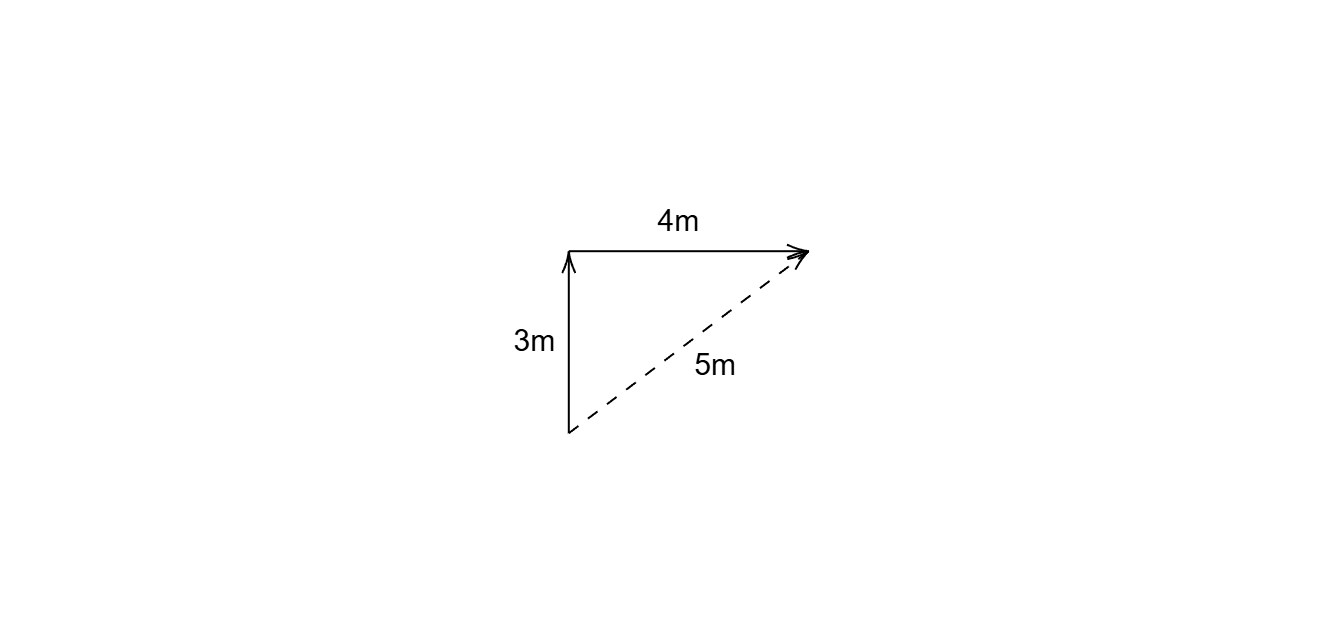
\includegraphics[width=1\textwidth]{Tuan2/Figures/gioithieuvector.png}
\end{figure}
Như vậy nhằm truyền tải những thông tin như vị trí của một vật, ta cần một mảng số (trong trường hợp vừa rồi là một mảng số có hai thành phần), hoặc một cách khác, là \emph{chỉ} về vật thể và xác định rõ ràng khoảng cách. Rõ ràng là kiểu thông tin này không giống với "quãng đường cần đi là 7m", hay "nhiệt độ hôm nay là 30 độ C", được truyền tải thông qua chỉ một con số (và dơn vị). Ta cần một đại lượng có khả năng truyền tải nhiều thông tin hơn để mô tả những 
dạng thông tin phức tạp hơn vậy. Nó được gọi là \textbf{vector}.
\begin{definition} Vector \(AB\) (hình vẽ), kí hiệu là \(\mathbf{AB}\), là một đại lượng biểu diễn bằng mũi tên tuân theo quy tắc hình bình hành được đặc trưng bởi độ dài \(a\) của nó (do đó còn được kí hiệu là \(\vec{a}\)) và hướng mà nó chỉ.
\end{definition}
\begin{figure}[H]
\centering

\includegraphics[width=1\textwidth]{Tuan2/Figures/vectorAB.png}
\end{figure}Đây là một định nghĩa thuần tuý hình học, nhưng sẽ ổn nếu bắt đầu với nó. Một mũi tên chỉ hướng với độ dài xác định là tương đương với một mảng số, như được trình bày trong ví dụ trên. Trong phần này, ta sẽ chủ yếu tập trung vào ý nghĩa hình học của vector , trực quan và không đi sâu vào khía cạnh toán.
Chỉ với định nghĩa này, các đại lượng phức tạp như lực, vận tốc cũng đã có thể được mô tả. Rõ ràng, chúng không thể được xác định chỉ với một con số như khối lượng hay nhiệt độ; vận tốc, lực, hay bất kỳ một đại lượng vector nào khác trong vật lý đều có \emph{hướng} và \emph{độ lớn}. Sau đây ta cũng thống nhất sẽ kí hiệu vector là \(\mathbf{a}\) thay vì \(\vec a\).
\vspace{8pt}

Để so sánh hai vector, ta dựa trên các tiêu chí sau:
    \begin{itemize}
        \item Hai vector \(\mathbf{a}\) và \(\mathbf{b}\) được coi là bằng nhau nếu chúng có cùng độ dài và cùng hướng, kí hiệu là \(\mathbf{a}=\mathbf{b}\).
        \item Hai vector \(\mathbf{a}\) và \(\mathbf{b}\) là đồng phương nếu chúng song song.
        \item Hai vector \(\mathbf{a}\) và \(\mathbf{b}\) có cùng giá nếu chúng cùng nằm trên một đường thẳng, và là đồng phẳng nếu cùng nằm trên một mặt phẳng.
    \end{itemize}

Ngoài ra, để kí hiệu độ lớn của một vector, ta viết \(\lvert \mathbf{a}\rvert\), ngắn gọn là \(a\) nếu không có gì nhầm lẫn.  
\subsection{Các phép toán trên vector}

\subsubsection{Phép cộng vector}
Tưởng tượng để xác định vị trí của viên đá, thay vì xác định trực tiếp, bạn xác định vị trí của Hirrus, và Hirrus xác định vị trí của viên đá. Từ đó, vị trí của nhân vật này được xác định bởi một vector có gốc ở vị trí của ta, đầu ở chỗ của Hirrus; vị trí của viên đá đối với Hirrus lại được xác định bởi một mũi tên có gốc đặt tại chỗ của Hirrus, đầu ở chỗ của viên đá. Đồng thời, vị trí của viên đá đối với bạn được xác định bởi một mũi tên có gốc ở vị trí của bạn, đầu ở chỗ của viên đá. Mũi tên này là kết quả của phép cộng hai mũi tên trước đó, và được gọi là \textbf{phép cộng vector}.
\begin{figure}[H]
    \centering
    \includegraphics[width=1\textwidth]{Tuan2/Figures/congvector.png}
    \caption{$\mathbf{a}+\mathbf{b}+\mathbf{c}+\mathbf{d}=\mathbf{AB}$}
\end{figure}
Chú ý rằng, về tổng quát, \(\lvert \mathbf{a}+\mathbf{b}\rvert\neq a+b\).
\subsubsection{Tích một vector với một đại lượng vô hướng}
Khi nhân một vector với một đại lượng vô hướng, độ dài của vector sẽ được nhân lên với hệ số bằng đại lượng đó, trong khi hướng của vector không đổi nếu số đó là số dương, đảo chiều nếu số đó là số âm. Đặc biệt, nếu một vector nhân với \(0\), kết quả là vector \(\mathbf{0}=\mathbf{a}+(-\mathbf{a})\).
\begin{figure}[H]
    \centering
    
\includegraphics[width=1\textwidth]{Tuan2/Figures/vector x vo huong.png}
    \caption{phép nhân vector với một đại lượng vô hướng}
\end{figure}

\subsubsection{Tích vô hướng hai vector}
Phép nhân vô hướng hai vector \(\mathbf{a}\) và \(\mathbf{b}\) có kết quả là một đại lượng vô hướng có giá trị bằng:
\begin{equation}
    \mathbf{a} \cdot \mathbf{b} = |\mathbf{a}| |\mathbf{b}| \cos (\mathbf{a}, \mathbf{b})
\end{equation}
Trong đó, \(\cos (\mathbf{a}, \mathbf{b})\) chỉ góc giữa hai vector \(\mathbf{a} \text{ và }\mathbf{b}\).
Ý nghĩa của phép nhân vô hướng được thể hiện như hình vẽ:
\begin{figure}[H]
    \centering
    \includegraphics[width=1\textwidth]{Tuan2/Figures/tichcham.png}
    \caption{phép nhân vô hướng hai vector}
\end{figure}
\subsubsection{Tích có hướng hai vector}
Phép nhân có hướng hai vector \(\mathbf{a}\) và \(\mathbf{b}\) có kết quả là một vector hướng vuông góc với mặt phẳng chứa hai vector này:
\begin{figure}[H]
    \centering
    
\includegraphics[width=1\textwidth]{Tuan2/Figures/tichcheo.png}
    \caption{phép nhân có hướng hai vector}
\end{figure}
Vector này có độ dài bằng:
\begin{equation}
    |\mathbf{a} \times \mathbf{b}| = |\mathbf{a}| |\mathbf{b}| \sin (\mathbf{a}, \mathbf{b})
\end{equation}
Chiều của vector này, theo quy ước,  được xác định bằng quy tắc bàn tay phải, hoặc quy tắc vặn nút chai (như hình vẽ).


\subsection{Đạo hàm vector}
\begin{definition}
    Cho \(\mathbf{u}(t)\) là một hàm vector. Đạo hàm của hàm vector này tại điểm \(t_0\) được định nghĩa là:
    \begin{equation}
        \mathbf{u}'(t_0) = \lim_{t \to t_0} \frac{\mathbf{u}(t) - \mathbf{u}(t_0)}{t - t_0}
    \end{equation}
\end{definition}
Cũng giống như đạo hàm của một hàm số, đạo hàm của một hàm vector cũng có một số tính chất đặc biệt:
\begin{itemize}
\item Nếu \(\mathbf{w}(t)=a(t)\mathbf{u}(t)\), thì \(\dfrac{d\mathbf{w}}{dt} = a'(t)\mathbf{u}(t) + a(t)\dfrac{d\mathbf{u}}{dt}\)
\item Nếu \(\mathbf{w}(t)=\mathbf{u}(t) + \mathbf{v}(t)\), thì \(\dfrac{d\mathbf{w}}{dt} = \dfrac{d\mathbf{u}}{dt} + \dfrac{d\mathbf{v}}{dt}\)
\item Nếu \(\mathbf{w}(t)=\mathbf{u}(t) \cdot \mathbf{v}(t)\), thì \(\dfrac{d\mathbf{w}}{dt} = \dfrac{d\mathbf{u}}{dt} \cdot \mathbf{v}(t) + \mathbf{u}(t) \cdot \dfrac{d\mathbf{v}}{dt}\)
\item Nếu \(\mathbf{w}(t)=\mathbf{u}(t) \times \mathbf{v}(t)\), thì \(\dfrac{d\mathbf{w}}{dt} = \dfrac{d\mathbf{u}}{dt} \times \mathbf{v}(t) + \mathbf{u}(t) \times \dfrac{d\mathbf{v}}{dt}\)
\end{itemize}

\subsection{Cơ sở vector}
\subsubsection{Vector đơn vị}
Một vector đơn vị là một vector có độ dài bằng 1. Vector đơn vị thường được sử dụng để biểu diễn hướng của một vector khác. Ví dụ, nếu \(\mathbf{a}\) là một vector bất kỳ, thì vector đơn vị theo hướng của \(\mathbf{a}\) được tính bằng:
\begin{equation}
    \mathbf{u} = \frac{\mathbf{a}}{|\mathbf{a}|} 
\end{equation}
Vector này có độ dài bằng 1 và cùng hướng với \(\mathbf{a}\).
\subsubsection{Cơ sở vector}
Trong không gian ba chiều, một vector cơ sở chuẩn hóa là tập hợp của ba vector đơn vị không đồng phẳng. Một vector có thể được xác định bằng cách biểu diễn nó dưới dạng tổ hợp tuyến tính của các vector đơn vị trong cơ sở.
\begin{equation}
    \mathbf{u}=a\mathbf{e}_1+b\mathbf{e}_2+c\mathbf{e}_3
\end{equation}
\begin{figure}[H]
    \centering
    \includegraphics[width=1\textwidth]{Tuan2/Figures/cosovector.png}
    \caption{Cơ sở \((\mathbf{e}_1, \mathbf{e}_2, \mathbf{e}_3)\)}
\end{figure}
Tương tự, trong không gian hai chiều, một vector cơ sở chuẩn hóa là tập hợp của hai vector đơn vị không nằm trên cùng một đường thẳng. Một vector trong mặt phẳng có thể được biểu diễn dưới dạng tổ hợp tuyến tính của các vector đơn vị trong cơ sở:
\[\mathbf{v}=a\mathbf{e}_1 +b\mathbf{e}_2.\]
Xét một vector khác, \(\mathbf{w}=c\mathbf{e}_1 +d\mathbf{e}_2\), vậy \[\mathbf{v}+\mathbf{w}=(a+c)\mathbf{e}_1 +(b+d)\mathbf{e}_2 .\]
Điều này nghĩa là, để đến vị trí được xác định bởi vector \(\mathbf{v}+\mathbf{w}\), ta đi từ vị trí ban đầu theo hướng của \(\mathbf{e}_1\) một khoảng bằng \(a+c\), rồi theo hướng của \(\mathbf{e}_2\) một khoảng bằng \(b+d\). Quay lại ví dụ ban đầu, ta thấy rằng nếu biết sẵn thông tin của \(\mathbf{e}_1\) và \(\mathbf{e}_2\), \(\mathbf{v}+\mathbf{w}\) được xác định qua mảng số \((a+c,b+d)\); 
tương tự, có thể viết \(\mathbf{v}=(a,b)\) hay \(\mathbf{w}=(c,d)\) để \(\mathbf{v}+\mathbf{w}=(a+c,b+d)\). \(a\) và \(b\) được gọi là các \emph{toạ độ} của vector \(\mathbf{v}\), cũng như \(c\) và \(d\) được gọi là các toạ độ của \(\mathbf{w}\).
\vspace{8pt}

Chú ý rằng các vector cơ sở cũng có toạ độ. Cụ thể, \((1,0)\) là toạ độ của \(\mathbf{e}_1\), và (\(0,1\)) là toạ độ của \(\mathbf{e}_2\). Trong trường hợp ba chiều, \(\mathbf{e}_1\), \(\mathbf{e}_2\), và \(\mathbf{e}_3\) có toạ độ lần lượt là \((1,0,0), (0,1,0), (0,0,1)\).

\subsection{Hệ tọa độ Descartes}
\begin{definition}
    Hệ tọa độ Descartes là một hệ tọa độ trực chuẩn, được xác định bởi một gốc tọa độ \(O\) và một vector cơ sở trực chuẩn (\(\mathbf{e}_1, \mathbf{e}_2, \mathbf{e}_3\)). Trong hệ tọa độ này, một điểm \(M\) trong không gian được xác định bởi ba tọa độ \((x, y, z)=(r_1, r_2, r_3)\),
    \begin{equation}
        \mathbf{r}=\mathbf{OM} = x\mathbf{e}_1 + y\mathbf{e}_2 + z\mathbf{e}_3.
    \end{equation}
\end{definition}
\begin{figure}[H]
    \centering
    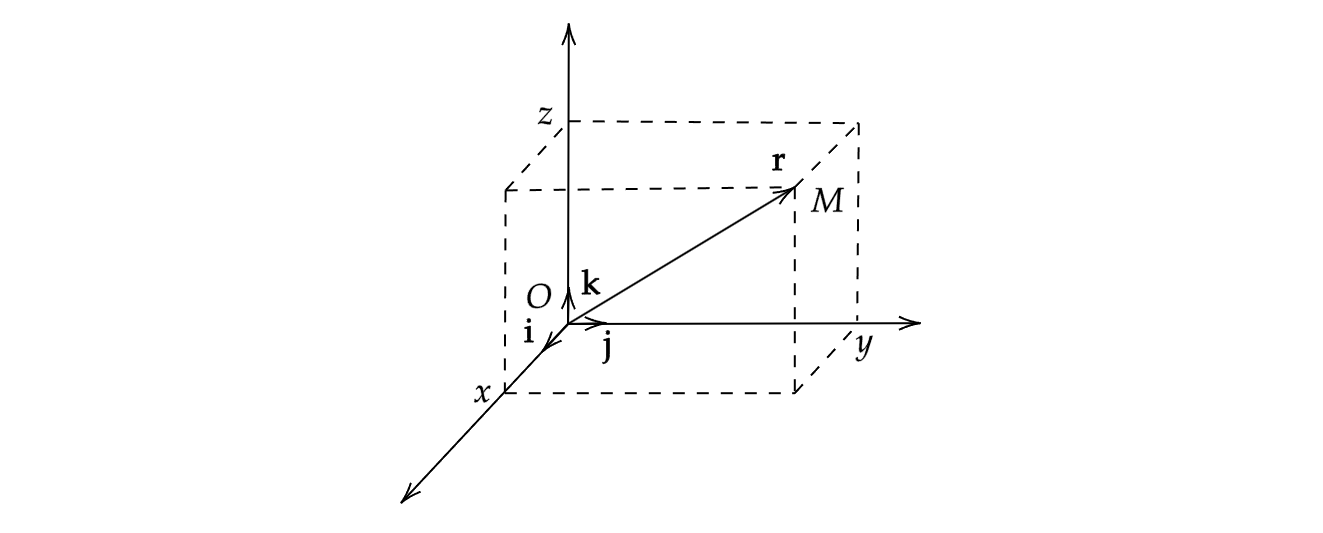
\includegraphics[width=1\textwidth]{Tuan2/Figures/toadodescartes.png}
    \caption{Hệ tọa độ Descartes}
\end{figure}
Trực chuẩn có nghĩa là các vector trong vector cơ sở có độ dài bằng 1 và vuông góc lẫn nhau. Nói cách khác, 
\begin{equation}
    \mathbf{e}_i \cdot \mathbf{e}_j =\delta_{ij}.
\end{equation}
Trong đó, \begin{equation*}
\begin{array}{l}
     \delta_{ij}=\Bigg\{
    \begin{array}{ll}
      1  & \text{, nếu } i=j. \\
      0  & \text{, nếu } i\neq j.
    \end{array}
\end{array}
\end{equation*} được gọi là ký hiệu Kronecker. Như vậy, tích vô hướng của hai vector \(\mathbf{a}=(a_1, a_2, a_3)\) và \(\mathbf{b}=(b_1,b_2,b_3)\) trong hệ tọa độ Descartes có thể được tính bằng công thức:
\begin{equation}
    \mathbf{a}\cdot\mathbf{b}=\sum_{i=1}^{3} a_m b_m = a_1 b_1 + a_2 b_2 + a_3 b_3.
\end{equation} Dễ thấy, \(\mathbf{a} \cdot \mathbf{e}_m =a_m\), nghĩa là thành phần thứ \(m\) của vector \(\mathbf{a}\) chính là tích vô hướng của \(\mathbf{a}\) với vector cơ sở thứ \(m\).
Đồng thời, ta cũng có 
\begin{align*}
\mathbf{e}_1 \times \mathbf{e}_1 = \mathbf{0},    && \mathbf{e}_1 \times \mathbf{e}_2 = \mathbf{e}_3,  && \mathbf{e}_1 \times \mathbf{e}_3 = -\mathbf{e}_2, \\
\mathbf{e}_2 \times \mathbf{e}_1 = -\mathbf{e}_3, && \mathbf{e}_2 \times \mathbf{e}_2 = \mathbf{0},    && \mathbf{e}_2 \times \mathbf{e}_3 = \mathbf{e}_1, \\
\mathbf{e}_3 \times \mathbf{e}_1 = \mathbf{e}_2,  && \mathbf{e}_3 \times \mathbf{e}_2 = -\mathbf{e}_1, && \mathbf{e}_3 \times \mathbf{e}_3 = \mathbf{0}.
\end{align*}
Tổng quát, tích có hướng của hai vector \(\mathbf{a}\) và \(\mathbf{b}\) bất kỳ có thể được viết thành
\begin{equation}
    \mathbf{a} \times \mathbf{b} = \sum_{i=1}^{3}\sum_{j=1}^{3}\sum_{k=1}^{3}\varepsilon_{ijk} a_i b_j  \mathbf{e}_k.
\end{equation}
Trong đó, \(\varepsilon_{ijk}\) là ký hiệu Levi-Civita, được định nghĩa như sau:
\begin{equation*}
\begin{array}{l}
        \varepsilon_{ijk}=\Bigg\{
        \begin{array}{ll}
        1  & \text{, nếu } (i,j,k)=(1,2,3) \text{ hoặc } (2,3,1) \text{ hoặc } (3,1,2).\\
        -1 & \text{, nếu } (i,j,k)=(1,3,2) \text{ hoặc } (2,1,3) \text{ hoặc } (3,2,1).\\
        0  & \text{, nếu } i=j \text{ hoặc } j=k \text{ hoặc } k=i.
        \end{array}
\end{array}
\end{equation*}  Đơn giản hơn, \[(\mathbf{a}\times\mathbf{b})_i = \sum_{j=1}^{3}\sum_{k=1}^{3}\varepsilon_{ijk}a_j b_k.\] Hay, 
\begin{equation}
    \mathbf{a}\times\mathbf{b}=(a_2 b_3 - a_3 b_2)\mathbf{e}_1 + (a_3 b_1 - a_1 b_3)\mathbf{e}_2 + (a_1 b_2 - a_2 b_1)\mathbf{e}_3.
\end{equation}


\subsection{Các phép toán với vector}
\begin{frame}
    \frametitle{Phép cộng vector}
    \begin{columns}
    \begin{column}{0.5\textwidth}
        Để xác định vị trí của viên đá, thay vì xác định trực tiếp, ta sẽ để Hirrus xác định vị trí của viên đá, rồi ta sẽ xác định vị trí của Hirrus.
        \begin{figure}
            \centering
            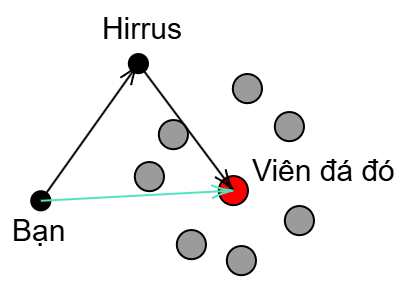
\includegraphics[width=0.7\textwidth]{Slides/Figure/HirrusAndStones.png}
        \end{figure}
    \end{column}
    \begin{column}{0.5\textwidth}
        \(\longrightarrow\) \textbf{Phép cộng vector}:
        \begin{figure}[H]
            \centering
            \includegraphics[width=0.7\textwidth]{Slides/Figure/congvector.png}
            \caption{$\mathbf{a}+\mathbf{b}+\mathbf{c}+\mathbf{d}=\mathbf{AB}$}
        \end{figure}
        Về tổng quát, \(|\mathbf a +\mathbf b| \neq a+b\).
        \end{column}
    \end{columns}
\end{frame}
\begin{frame}
    \frametitle{Phép nhân vector-vô hướng}
    \begin{itemize}
        \item \(\lvert n\mathbf{a}\rvert =\lvert n\rvert \lvert \mathbf{a}\rvert .\)
        \item \(0\mathbf{a}=\mathbf{0}\).
        \item \(-1\mathbf{a}=-\mathbf{a}\).
    \end{itemize}
    \begin{figure}[H]
        \centering
        
\includegraphics[width=12cm, height=3cm]{Slides/Figure/vector x vo huong.png}
    \end{figure}
\end{frame}
\begin{frame}
\frametitle{Hai phép nhân vector-vector}
\begin{columns}
\begin{column}{0.5\textwidth}
    \textbf{Phép nhân vô hướng hai vector}
    \begin{figure}
    \centering
    \includegraphics[width=0.65\textwidth]{Slides/Figure/tichcham.png}
    \end{figure}
    \begin{itemize}
        \item Kết quả là một số vô hướng.
        \item \(\mathbf a \cdot \mathbf b = ab \cos \alpha\)
    \end{itemize}
\end{column}
\begin{column}{0.5\textwidth}
    \textbf{Phép nhân có hướng hai vector}
    \begin{figure}
    \centering
    
\includegraphics[width=0.5\textwidth]{Slides/Figure/tichcheo.png}
    \end{figure}
    \begin{itemize}
        \item Kết quả là một vector.
        \item \(|\mathbf a \times \mathbf b| = ab \sin \alpha\)
    \end{itemize}
\end{column}
\end{columns}
\end{frame}
\subsection{Cơ sở vector và hệ tọa độ}
\begin{frame}
\frametitle{Vector đơn vị}
\begin{tcolorbox}[colback=blue!10, colframe=blue!50!black, title=Định nghĩa]
    Một vector đơn vị là một vector có độ dài bằng 1. Ví dụ, nếu \(\mathbf{a}\) là một vector bất kỳ, thì vector đơn vị theo hướng của \(\mathbf{a}\) được tính bằng:
\begin{equation}
    \mathbf{u} = \frac{\mathbf{a}}{|\mathbf{a}|} 
\end{equation}
Vector này có độ dài bằng 1 và cùng hướng với \(\mathbf{a}\).
\end{tcolorbox}
\end{frame}

\begin{frame}
\frametitle{Cơ sở vector}
\begin{tcolorbox}[colback=blue!10, colframe=blue!50!black, title=Định nghĩa]
    Một vector cơ sở chuẩn hóa là một tập hợp các vector độc lập tuyến tính mà mọi vector trong không gian có thể được biểu diễn như một tổ hợp tuyến tính của các vector trong cơ sở đó.
\end{tcolorbox}
\end{frame}

\begin{frame}
\frametitle{Cơ sở vector}
\begin{columns}
\begin{column}{0.5\textwidth}
Trong không gian ba chiều, một vector cơ sở chuẩn hóa là tập hợp của ba vector đơn vị không đồng phẳng. Một vector có thể được xác định bằng cách biểu diễn nó dưới dạng tổ hợp tuyến tính của các vector đơn vị trong cơ sở.
\begin{equation}
    \mathbf{u}=a\mathbf{e}_1+b\mathbf{e}_2+c\mathbf{e}_3
\end{equation}
\end{column}
\begin{column}{0.5\textwidth}
\begin{figure}
\centering
\includegraphics[width=0.9\textwidth]{Slides/Figure/cosovector.png}
\caption{Cơ sở \((\mathbf{e}_1, \mathbf{e}_2, \mathbf{e}_3)\)}
\end{figure}
\end{column}
\end{columns}
\end{frame}

\begin{frame}
\frametitle{Hệ tọa độ Descartes}
\begin{tcolorbox}[colback=blue!10, colframe=blue!50!black, title=Định nghĩa]
    Hệ tọa độ Descartes là một hệ tọa độ trực chuẩn, được xác định bởi một gốc tọa độ \(O\) và một vector cơ sở trực chuẩn (\(\mathbf{e}_1, \mathbf{e}_2, \mathbf{e}_3\)). Trong hệ tọa độ này, một điểm \(M\) trong không gian được xác định bởi ba tọa độ \((x, y, z)=(r_1, r_2, r_3)\),
    \begin{equation}
        \mathbf{r}=\mathbf{OM} = x\mathbf{e}_1 + y\mathbf{e}_2 + z\mathbf{e}_3.
    \end{equation}
\end{tcolorbox}
\end{frame}

\begin{frame}
\frametitle{Hệ tọa độ Descartes}
\begin{figure}
\centering
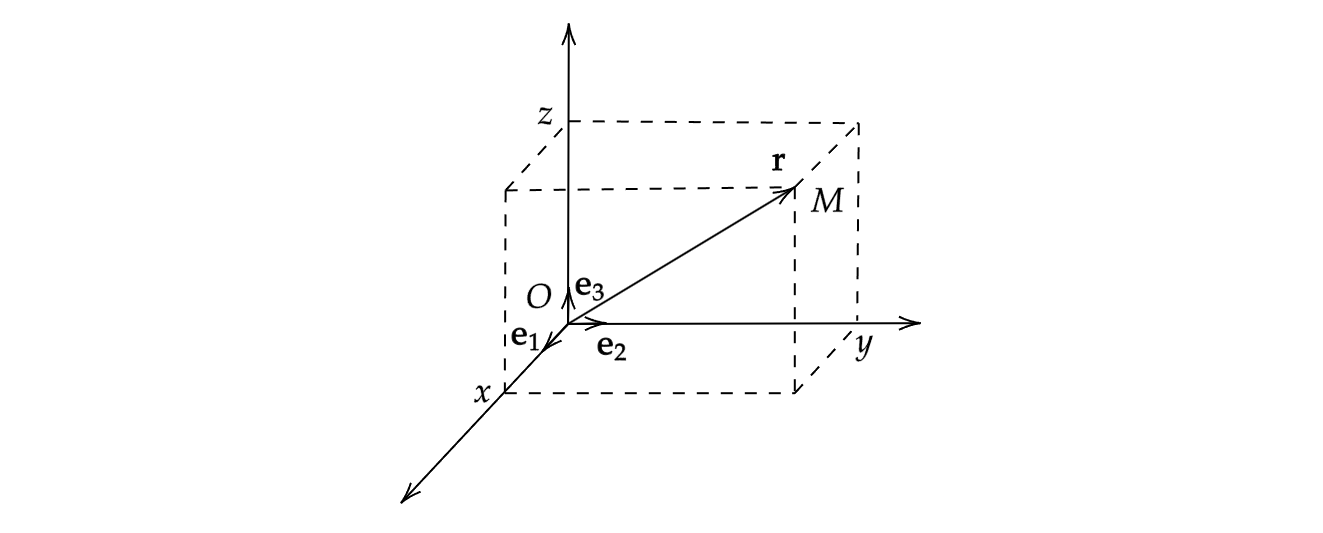
\includegraphics[width=1\textwidth]{Slides/Figure/toadodescartes.png}
\caption{Hệ tọa độ Descartes \(Oxyz\)}
\end{figure}
\end{frame}
\section{Vector và\ldots nhiều vector hơn}
\subsection{Không gian vector}
\begin{frame}
    \frametitle{Cơ sở}
    Cho hai hệ cơ sở:
               \begin{itemize}
                  \item \((\mathbf{e}_1 ,\mathbf{e}_2)\) 
                \item \((\mathbf{e}_3 ,\mathbf{e}_4)\) 
                \end{itemize}
                \(\implies \mathbf{v}=\alpha\mathbf{e}_1 +\beta\mathbf{e}_2 =\gamma\mathbf{e}_3 +\sigma\mathbf{e}_{4}.\)
\end{frame}
\begin{frame}
    \frametitle{Cơ sở}
    \begin{columns}
        \begin{column}{0.45\textwidth}
            Cho hai hệ cơ sở:
               \begin{itemize}
                  \item \((\mathbf{e}_1 ,\mathbf{e}_2)\) 
                \item \((\mathbf{e}_3 ,\mathbf{e}_4)\) 
                \end{itemize}
                \(\implies \mathbf{v}=\alpha\mathbf{e}_1 +\beta\mathbf{e}_2 =\gamma\mathbf{e}_3 +\sigma\mathbf{e}_{4}.\)

                Giả sử: 
                \begin{itemize}
                \item \(\mathbf{e}_3 =2\mathbf{e}_1 -3\mathbf{e}_2 ,~\mathbf{e}_4 =\mathbf{e}_1 +2\mathbf{e}_2\),
                \item \(\alpha=5, \beta =3\).
                \end{itemize}
                \(\implies \mathbf{v}=\mathbf{e}_3 +3\mathbf{e}_4\).
        \end{column}
        \begin{column}{0.55\textwidth}
            Nếu \(\mathbf{e}_1 ,\mathbf{e}_2\) trực chuẩn:
            \begin{figure}[htps]
                \centering
                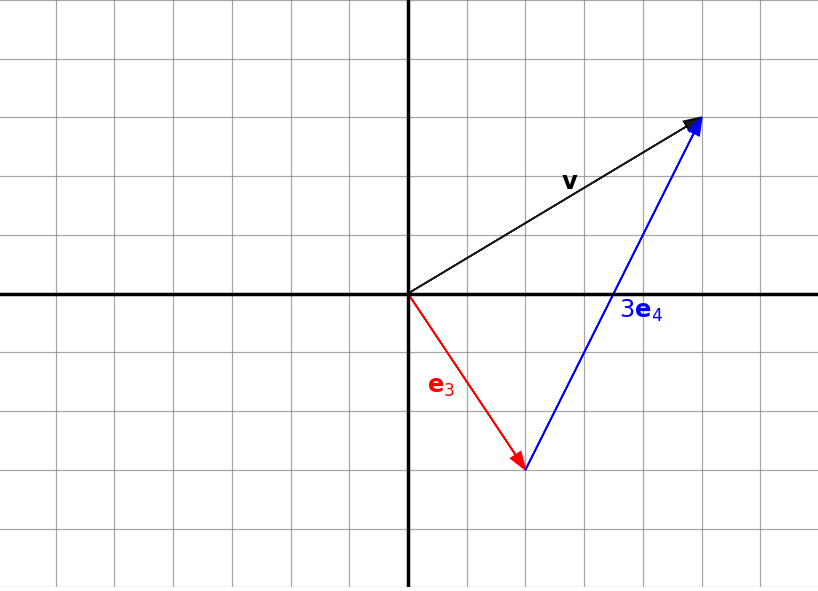
\includegraphics[width=7cm, height=5.5cm]{Slides/Figure/e3e4.png}
            \end{figure}
        \end{column}
    \end{columns}
\end{frame}
\begin{frame}
    \frametitle{Cơ sở}
    Nếu thay vì \((\mathbf{e}_3 ,\mathbf{e}_4)\), ta chọn (\(\mathbf{e}_3 ,2\mathbf{e}_3\)) thì sao?
\end{frame}
\begin{frame}
    \frametitle{Cơ sở}
    Nếu thay vì \((\mathbf{e}_3 ,\mathbf{e}_4)\), ta chọn (\(\mathbf{e}_3 ,2\mathbf{e}_3\)) thì sao?
    \begin{figure}[H]
        \centering
        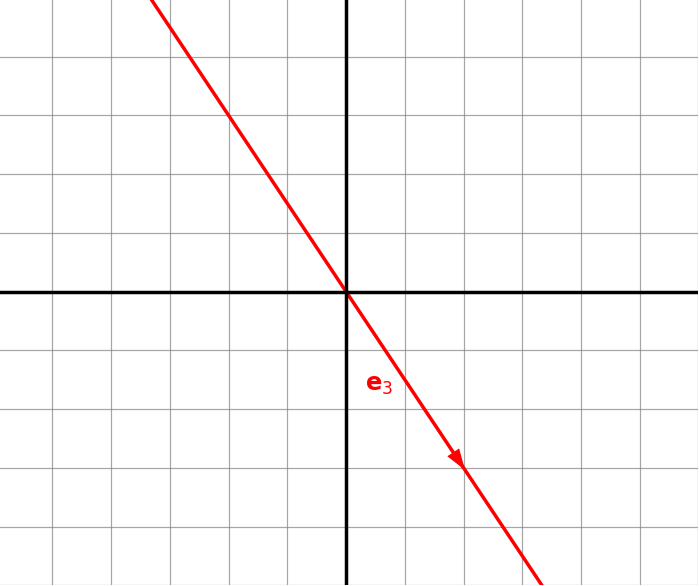
\includegraphics[width=7cm, height=6cm]{Slides/Figure/avectoronaline.png}
    \end{figure}
\end{frame}
\begin{frame}
    \frametitle{Định nghĩa}
    \begin{tcolorbox}[colback=blue!10!, colframe=blue!50!black, title=Bao tuyến tính]
        Nếu \(S=\{\mathbf{u}_{1}, \mathbf{u}_{2},\dots,  \mathbf{u}_{n}\}\) là một tập hợp \(n\) vector trong không gian, thì tập hợp tất cả các tổ hợp tuyến tính của chúng được gọi là bao tuyến tính của \(\mathbf{u}_{1}, \mathbf{u}_{2},\dots \mathbf{u}_{n}\), và được kí hiệu là span(\(S\)).
       \vspace{8pt}

        Nếu span(S) chứa toàn bộ vector trong không gian, vậy ta gọi S là một hệ sinh cho không gian.
    \end{tcolorbox}
\end{frame}
\begin{frame}
\frametitle{Định nghĩa}
    \begin{tcolorbox}[colback=blue!10!, colframe=blue!50!black, title=Độc lập tuyến tính]
        Một tập hợp các vector được gọi là \emph{độc lập tuyến tính} với nhau nếu tổ hợp tuyến tính của chúng không bao giờ bằng \(\mathbf{0}\) trừ khi \textbf{tất cả} các hệ số vô hướng đều bằng \(0\).
    \end{tcolorbox}
\end{frame}
\begin{frame}
\frametitle{Định nghĩa}
    \begin{tcolorbox}[colback=blue!10!, colframe=blue!50!black, title=Hệ cơ sở]
        Một cơ sở của không gian là một tập hợp các vector trong không gian sao cho 
    \begin{itemize}
        \item tạo thành hệ sinh cho không gian, và
        \item độc lập tuyến tính.
    \end{itemize}
    \end{tcolorbox}
\end{frame}
\begin{frame}
    \frametitle{Ví dụ}
    \begin{columns}
        \begin{column}{0.5\textwidth}
        Hệ sinh của mặt phẳng đã được đề cập:
        \begin{itemize}
            \item \(S_1=\{\mathbf{e}_1 ,\mathbf{e}_2\}\),
            \item \(S_2 =\{\mathbf{e}_3 ,\mathbf{e}_4\}\),
            \item \(S_3 =\{\mathbf{e}_3 ,\mathbf{e}_4 ,2\mathbf{e}_3\}\).
        \end{itemize}
        \end{column}
        \begin{column}{0.5\textwidth}
            Hệ sinh của đường thẳng chứa \(\mathbf{e}_3\):
            \begin{itemize}
                \item \(S_1 =\{\mathbf{e}_3\}\),
                \item \(S_2 =\{\mathbf{e}_3 ,2\mathbf{e}_3\}\),
                \item \(S_2 =\{\mathbf{e}_3 ,2\mathbf{e}_3 ,\mathbf{0}\}\).
            \end{itemize}
        \end{column}
        \end{columns}
    \vspace{10pt}

    \begin{columns}
        \begin{column}{0.5\textwidth}
            Nhưng,
            \begin{itemize}
                \item (\(\mathbf{e}_3 ,\mathbf{e}_4 ,2\mathbf{e}_3\))
            \end{itemize}
            không phải là một hệ cơ sở.
        \end{column}
        \begin{column}{0.5\textwidth}
            Nhưng,
            \begin{itemize}
                \item (\(\mathbf{e}_3 ,2\mathbf{e}_3\)), và
                \item (\(\mathbf{e}_3 ,\mathbf{0}\))
            \end{itemize}
            không phải là một hệ cơ sở.
        \end{column}
    \end{columns}
\end{frame}
\begin{frame}
    \frametitle{Ví dụ}
    Vì:
    \begin{itemize}
         \item   \(-2\mathbf{e}_{3}+1(2\mathbf{e}_{3})+0\mathbf{e}_{4}=\mathbf{0}\),
           \item \(-2\mathbf{e}_{3}+1(2\mathbf{e}_{3})=\mathbf{0}\),
        \item    \(0\mathbf{e}_3 +100(\mathbf{0})=\mathbf{0}\).
    \end{itemize}
\end{frame}
\begin{frame}
    \frametitle{Không gian vector}
    Có một sự mập mờ khi sử dụng cụm từ "không gian" trong các phần trước!
\end{frame}
\begin{frame}
    \frametitle{Không gian vector}
    Một không gian vector là một tập hợp mà các phần tử trong đó thoả mãn:
    \begin{enumerate}
        \item Với mọi \(\mathbf{v}, \mathbf{w}\in V , \mathbf{v}+\mathbf{w}\in V\).
        \item Với mọi \(\mathbf{v}\in V, \alpha\in \mathbb{R}, \alpha\mathbf{v}\in V\).
        \item \(\mathbf{v}+\mathbf{w}=\mathbf{w}+\mathbf{v}\).
        \item   \(\mathbf{u}+(\mathbf{v}+\mathbf{w})=(\mathbf{u}+\mathbf{v})+\mathbf{w}\).
        \item Tồn tại một vector \(\mathbf{0}\) sao cho \(\mathbf{v}+\mathbf{0}=\mathbf{v}\).
        \item Với mọi vector \(\mathbf{v}\), tồn tại một vector \(\mathbf{v}'\) sao cho \(\mathbf{v}+\mathbf{v}'=\mathbf{0}\).
        \item \(1\mathbf{v}=\mathbf{v}\).
        \item \(\alpha(\beta\mathbf{v})=(\alpha\beta)\mathbf{v}\).
        \item \(\alpha(\mathbf{v}+\mathbf{w})=\alpha\mathbf{v}+\alpha\mathbf{w}\).
        \item \((\alpha+\beta)\mathbf{v}=\alpha\mathbf{v}+\beta\mathbf{v}\). 
    \end{enumerate}
\end{frame}
\begin{frame}
    \frametitle{Ví dụ 1}
    Tập hợp số thực: \(\mathbb{R}^1\)
    \begin{figure}[H]
        \centering
        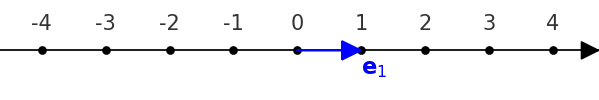
\includegraphics[width=12cm, height=2cm]{Slides/Figure/1Dvectorspace.png}
    \end{figure}
    Vector: \(-1.9, 5, 2,100, -\pi, e,\dots\)
\end{frame}
\begin{frame}
    \frametitle{Ví dụ 2}
    Mặt phẳng toạ độ: \(\mathbb{R}^2\)
    \begin{figure}[H]
        \centering
        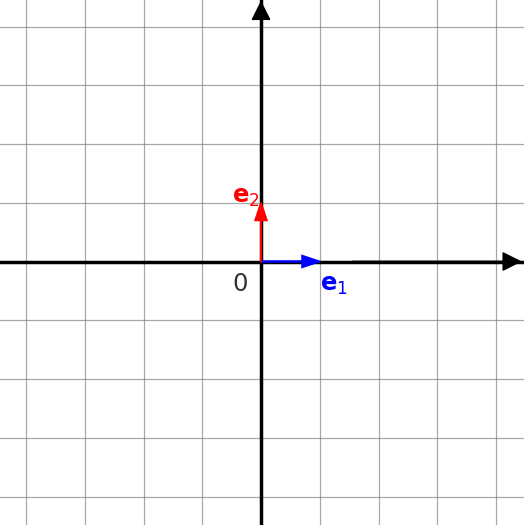
\includegraphics[width=6cm, height=4.5cm]{Slides/Figure/2Dvectorspace.png}
    \end{figure}
    Vector: \((1.23;2),(\pi, e),(-111,-\pi),\dots\)
\end{frame}
\begin{frame}
    \frametitle{Ví dụ 3}
    Không gian hình học: \(\mathbb{R}^3\)
    \begin{figure}[H]
        \centering
        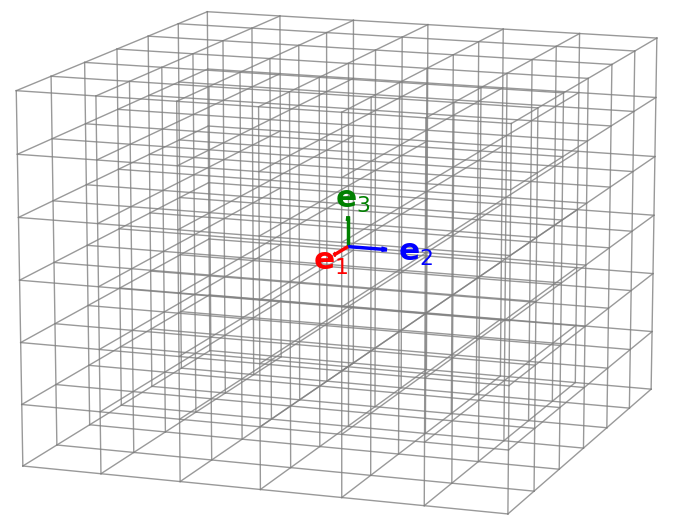
\includegraphics[width=6cm, height=4.5cm]{Slides/Figure/3Dvectorspace.png}
    \end{figure}
    Vector: \((1;3;4),(100,0,0),\dots\)
\end{frame}
\begin{frame}
    \frametitle{Chiều}
    \begin{tcolorbox}[colback=blue!10!, colframe=blue!50!black, title=Chiều của không gian vector]
        Chiều của một không gian là số lượng vector trong hệ cơ sở của không gian đó.
    \end{tcolorbox}
    
\end{frame}
\begin{frame}
    \frametitle{Chiều}
    \begin{tcolorbox}[colback=blue!10!, colframe=blue!50!black, title=Chiều của không gian vector]
        Chiều của một không gian là số lượng vector trong hệ cơ sở của không gian đó.
    \end{tcolorbox}
    \(\mathbb{R}, \mathbb{R}^2 ,\mathbb{R}^3\) đã được đề cập. Vậy \(\mathbb{R}^4, \mathbb{R}^5 ,\cdots\) thì sao?
\end{frame}
\begin{frame}
    \frametitle{Chiều}
    Vector trong   \(\mathbb{R}^4\): Mảng số có 4 thành phần.
 
    Vector trong \(\mathbb{R}^5\): Mảng số có 5 thành phần.

    \dots

    Vector trong \(\mathbb{R}^{100}\): Mảng số có 100 thành phần.
    
    Vector trong \(\mathbb{R}^{\text{n}}\): Mảng số có n thành phần!
    \begin{figure}
        \centering
        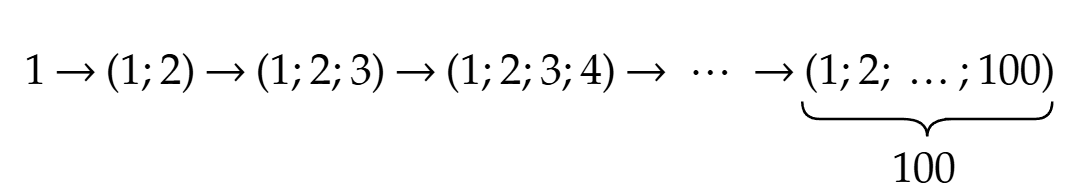
\includegraphics[width=12cm, height=2cm]{Slides/Figure/1to100.png}
    \end{figure}
\end{frame}
\begin{frame}
    \frametitle{Mũi tên hay mảng số?}
    Từ \(\mathbb{R}^4\) trở đi, không còn mũi tên nào cả.
    \begin{figure}
        \centering
        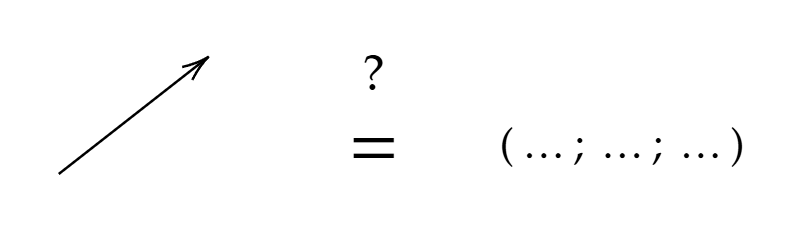
\includegraphics[width=12cm, height=3cm]{Slides/Figure/arroworarray.png}
    \end{figure}
\end{frame}
\begin{frame}
    \frametitle{Vector?}
    \begin{itemize}
        \item \(\mathbb{C}^n : (1+2i; 0.76-100i; i; e+\pi i;\dots)\).
    \end{itemize}
\end{frame}
\begin{frame}
    \frametitle{Vector?}
    \begin{itemize}
        \item \(\mathbb{C}^n : (1+2i; 0.76-100i; i; e+\pi i;\dots)\).
        \item \(f(x)=1+2x^2 -3x^3 +42x^4\).
        \item \(g(x)=\sin x\).
        \item \(\cdots\)
    \end{itemize}
\end{frame}
\begin{frame}
    \frametitle{Quay trở lại với các vector thực}
    \begin{figure}[H]
    \centering
    \begin{subfigure}[t]{0.4\textwidth}
        \centering
        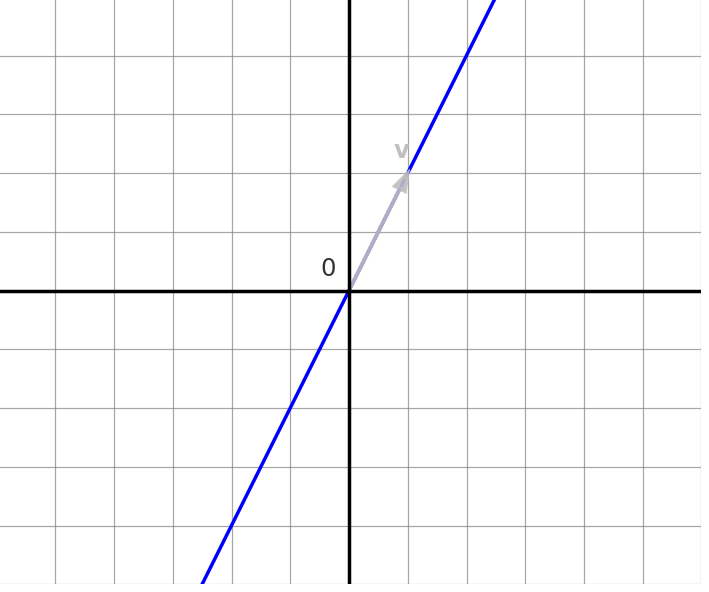
\includegraphics[width=5cm, height=5cm]{Slides/Figure/lineonplane.png}
        \caption{Đường thẳng (đi qua gốc toạ độ) trên mặt phẳng}
    \end{subfigure}
    \hfill
    \begin{subfigure}[t]{0.4\textwidth}
        \centering
        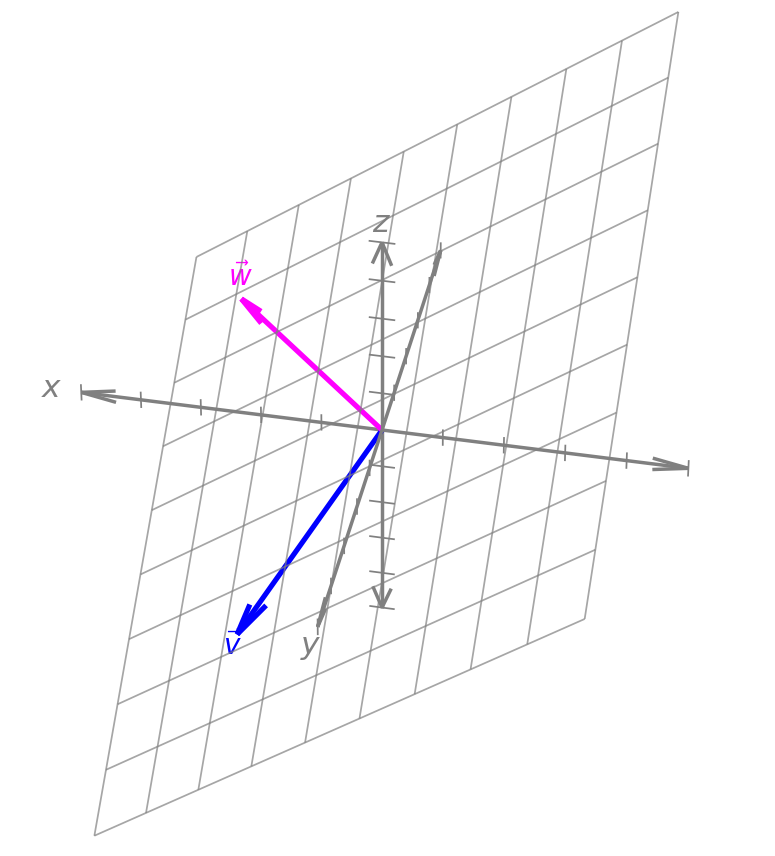
\includegraphics[width=5cm, height=5cm]{Slides/Figure/planeinspace.png}
        \caption{Mặt phẳng (đi qua gốc toạ độ) trong không gian}
    \end{subfigure}
\end{figure}
\end{frame}
\begin{frame}
    \frametitle{Không gian con}
    \begin{tcolorbox}[colback=blue!10!, colframe=blue!50!black, title=Không gian con]
        Một không gian con \(S\) trong một không gian vector \(V\) là một tập hợp các vector trong \(V\) sao cho chúng thoả mãn 10 tiên đề của vector.
    \end{tcolorbox}
    \begin{tcolorbox}[colback=blue!10!, colframe=blue!50!black, title=Cơ sở của không gian con]
        Một cơ sở cho một không gian con \(S\) của \(\mathbb{R}^n\) là một tập hợp các vector trong \(S\) sao cho 
    \begin{enumerate}
        \item tạo thành \(S\), và
        \item là độc lập tuyến tính.
    \end{enumerate}
    \end{tcolorbox}
\end{frame}
\begin{frame}
    \frametitle{Thêm ví dụ}
    Một đường thẳng đi qua gốc toạ độ trên một mặt phẳng trong không gian:
    \begin{figure}[H]
        \centering
        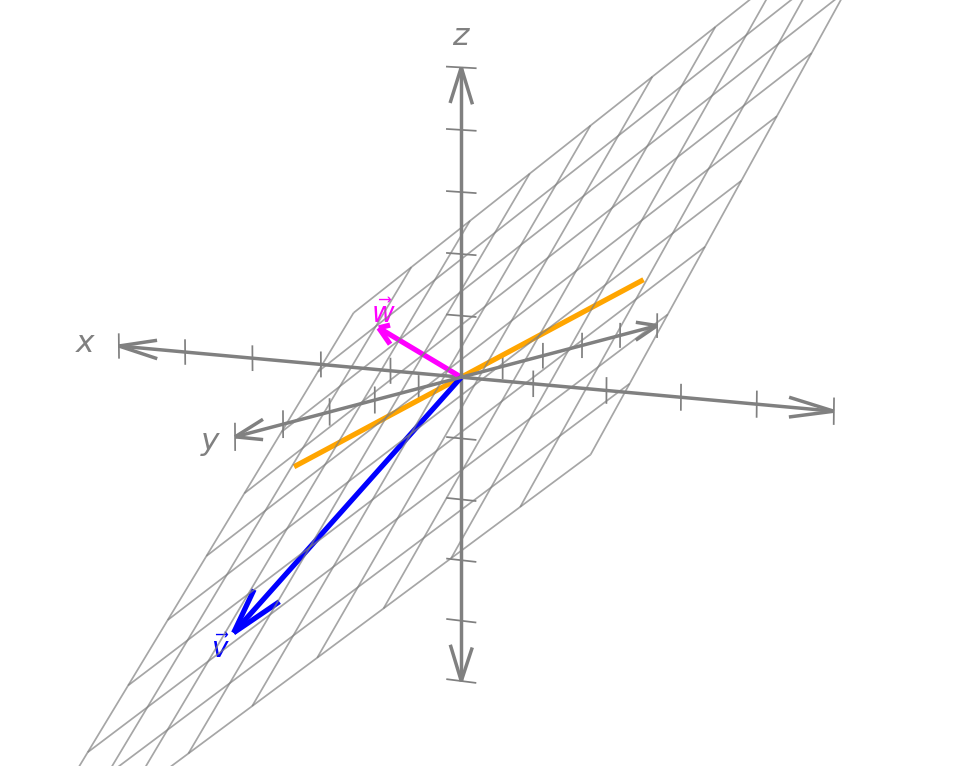
\includegraphics[width=7cm, height=5cm]{Slides/Figure/lineonplaneinspace.png}
    \end{figure}
\end{frame}
\subsection{Ma trận}
\begin{frame}
    \frametitle{Giới thiệu ma trận}
    \[ \mathbf{A}=
\begin{bmatrix}
    1&5&12\\
    3&0&4\\
    0&7&9
\end{bmatrix}
\]
\[\mathbf{B}=\begin{bmatrix}
    -1.3&0.6\\
    20.4&5.5\\
    9.7&-6.2
\end{bmatrix}\]
Quy tắc đọc: hàng trước cột sau.\newline
\(\mathbf{A}_{21}=3\).\newline
\(\mathbf{B}_{32}=-6.2\).
\end{frame}
\begin{frame}
    \frametitle{Ma trận 1 cột}
    Ví dụ:
    \[\mathbf{v}=\begin{bmatrix}
    a\\b\\c
\end{bmatrix}, \quad \mathbf{w}=\begin{bmatrix}
    c\\d\\f
\end{bmatrix}.\]
\end{frame}
\begin{frame}
    \frametitle{Ma trận 1 cột}
    Ví dụ: 
    \[\mathbf{v}=\begin{bmatrix}
    a\\b\\c
\end{bmatrix}, \quad \mathbf{w}=\begin{bmatrix}
    c\\d\\f
\end{bmatrix}.\]
Nếu,
\[\mathbf{v}+\mathbf{w}=\begin{bmatrix}
    a+c\\b+d\\c+f
\end{bmatrix},\qquad
    n\cdot\mathbf{v}=\begin{bmatrix}
        na\\nb\\nc
\end{bmatrix}.\] \[\implies \text{Vector}\]
\end{frame}
\begin{frame}
    \frametitle{Chuyển đổi ký hiệu}
    \[(a,b,c)\rightarrow \begin{bmatrix}
    a\\b\\c
\end{bmatrix}\]
\begin{figure}[H]
    \centering
    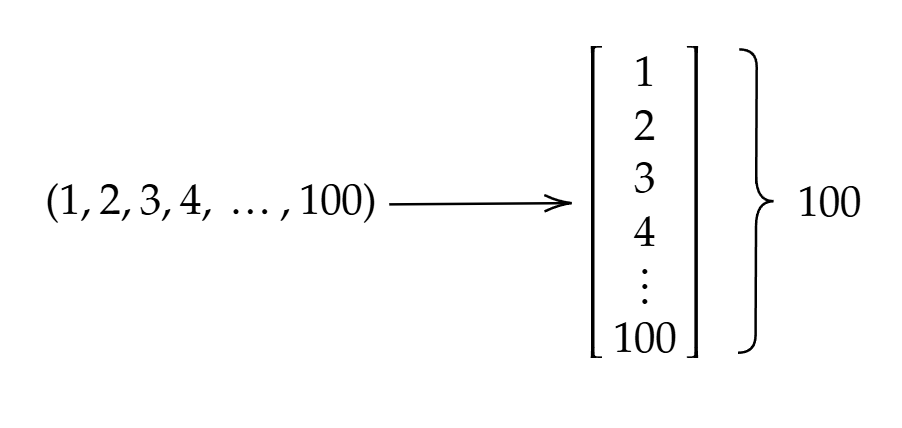
\includegraphics[width=9cm, height=4cm]{Slides/Figure/array100.png}
\end{figure}
\end{frame}
\begin{frame}
    \frametitle{Dạng tổng quát của một ma trận}
    Một ma trận m hàng n cột về tổng quát có dạng:
    \[\mathbf{A}_{m\times n}=\begin{bmatrix}
    \mathbf{A}_{11} &   \mathbf{A}_{12} &\cdots &\mathbf{A}_{1j} &\cdots      & \mathbf{A}_{1n}\\  
    \mathbf{A}_{21} &   \mathbf{A}_{22} &\cdots &\mathbf{A}_{2j} &\cdots      & \mathbf{A}_{2n}\\
    \vdots          &   \vdots          &\ddots &\vdots          &\ddots      & \vdots         \\
    \mathbf{A}_{i1} &   \mathbf{A}_{i2} &\cdots &\mathbf{A}_{ij} &\cdots      & \mathbf{A}_{in}\\
    \vdots          &   \vdots          &\ddots &\vdots          &\ddots      &\vdots          \\
    \mathbf{A}_{m1} &   \mathbf{A}_{m2} &\cdots &\mathbf{A}_{mj} &\cdots      & \mathbf{A}_{mn}              
\end{bmatrix}.\]
\end{frame}
\begin{frame}
    \frametitle{Các phép toán trên ma trận}
    \textbf{Phép cộng ma trận.} \[(\mathbf{A}+\mathbf{B})_{ij}=\mathbf{A}_{ij}+\mathbf{B}_{ij}.\]
    \textbf{Phép nhân ma trận với một số.}\[(c\mathbf{A})_{ij}=c\mathbf{A}_{ij}.\]
    Ví dụ: \[4\begin{bmatrix}
    0&3\\ 2&-6
\end{bmatrix}+\begin{bmatrix}
    1&-2\\ 0&5
\end{bmatrix}=??\]
\end{frame}
\begin{frame}
    \frametitle{Các phép toán trên ma trận}
    \textbf{Phép cộng ma trận.} \[(\mathbf{A}+\mathbf{B})_{ij}=\mathbf{A}_{ij}+\mathbf{B}_{ij}.\]
    \textbf{Phép nhân ma trận với một số.}\[(c\mathbf{A})_{ij}=c\mathbf{A}_{ij}.\]
    Ví dụ: \[4\begin{bmatrix}
    0&3\\ 2&-6
\end{bmatrix}+\begin{bmatrix}
    1&-2\\ 0&5
\end{bmatrix}=\begin{bmatrix}
    0&12\\ 8&-24
\end{bmatrix}+\begin{bmatrix}
    1&-2\\ 0&5
\end{bmatrix}=\begin{bmatrix}
    1&10\\ 8&-19
\end{bmatrix}.\]
\end{frame}
\begin{frame}
    \frametitle{Các phép toán trên ma trận}
    Cho \[\mathbf{v}=\begin{bmatrix}
    +2\\+5\\-4
\end{bmatrix}.\] Phân tích trong một hệ cơ sở ngẫu nhiên,
\[\begin{bmatrix}
    2\\5\\-4
\end{bmatrix}=\alpha\begin{bmatrix}
    1\\0\\0
\end{bmatrix}+\beta\begin{bmatrix}
    0\\2\\-5
\end{bmatrix}+\gamma\begin{bmatrix}
    0\\11\\-19
\end{bmatrix}.\]
\end{frame}
\begin{frame}
    \frametitle{Các phép toán trên ma trận}
    Cho \[\mathbf{v}=\begin{bmatrix}
    +2\\+5\\-4
\end{bmatrix}.\] Phân tích trong một hệ cơ sở ngẫu nhiên,
\[\begin{bmatrix}
    2\\5\\-4
\end{bmatrix}=\alpha\begin{bmatrix}
    1\\0\\0
\end{bmatrix}+\beta\begin{bmatrix}
    0\\2\\-5
\end{bmatrix}+\gamma\begin{bmatrix}
    0\\11\\-19
\end{bmatrix}.\]
Tính được \((\alpha,\beta,\gamma)=(2,-3,1)\).
\end{frame}
\begin{frame}
    \frametitle{Các phép toán trên ma trận}
    \textbf{Phép nhân ma trận-vector.}
    \[\begin{bmatrix}
    2\\5\\-4
\end{bmatrix}=2\begin{bmatrix}
    1\\0\\0
\end{bmatrix}+(-3)\begin{bmatrix}
    0\\2\\-5
\end{bmatrix}+1\begin{bmatrix}
    0\\11\\-19
\end{bmatrix}.\]
    \[\begin{bmatrix}
    2\\5\\-4
\end{bmatrix}=\begin{bmatrix}
    1&0&0\\
    0&2&11\\
    0&-5&-19
\end{bmatrix}\begin{bmatrix}
    2\\-3\\1
\end{bmatrix}.\]
\end{frame}
\begin{frame}
    \frametitle{Các phép toán trên ma trận}
    \textbf{Phép nhân ma trận-vector.}\begin{equation}\label{eq1}
    \begin{bmatrix}
    2\\5\\-4
\end{bmatrix}=\begin{bmatrix}
    1&0&0\\
    0&2&11\\
    0&-5&-19
\end{bmatrix}\begin{bmatrix}
    2\\-3\\1
\end{bmatrix}.\end{equation}
Một ma trận \(m\times n\) nhân với một vector n thành phần = một vector m thành phần; phần tử thú i của vector:
\begin{equation}
    (\mathbf{Ax})_i = \sum_{j=1}^n \mathbf{A}_{ij}\mathbf{x}_j.
\end{equation}
\end{frame}
\begin{frame}
    \frametitle{Phép nhân ma trận-vector}
    Phần tử thứ \(i\) của vector này là tích vô hướng của hàng thứ \(i\) của \(\mathbf{A}\) với vector \(\mathbf{x}\). Chẳng hạn,
    \[\begin{bmatrix}
    0&2&11
\end{bmatrix}\begin{bmatrix}
    2\\-3\\1
\end{bmatrix}=\begin{bmatrix}
    0\\2\\11
\end{bmatrix}\cdot \begin{bmatrix}
    2\\-3\\1
\end{bmatrix}=0\times 2+2\times(-3)+11\times 1 =5.\]
\end{frame}
\begin{frame}
    \frametitle{Phép nhân ma trận-vector}
    Tóm gọn:\[\begin{bmatrix}
    \vert &\vert&\vert\\
    \mathbf{A}_{i1}&\mathbf{A}_{i2}&\mathbf{A}_{i3}\\
    \vert &\vert&\vert\\
\end{bmatrix}\begin{bmatrix}
    x_1\\x_2\\x_3
\end{bmatrix}=x_1\begin{bmatrix}
    \vert\\\mathbf{A}_{i1}\\ \vert
\end{bmatrix}+x_2 \begin{bmatrix}
    \vert\\\mathbf{A}_{i2}\\ \vert
\end{bmatrix}+x_3\begin{bmatrix}
    \vert\\\mathbf{A}_{i1}\\ \vert
\end{bmatrix}.\]
Tính phân phối: \[\mathbf{A}(\mathbf{a}+\mathbf{b})=\mathbf{A}\mathbf{a}+\mathbf{A}\mathbf{b}.\]
\end{frame}
\begin{frame}
    \frametitle{Phép nhân ma trận với ma trận}
    \[
    \begin{bmatrix}
    1\\0\\0
    \end{bmatrix}=1\begin{bmatrix}
    0.5 \\-1\\0
    \end{bmatrix}+2\begin{bmatrix}
    0.75 \\1\\-2
    \end{bmatrix}+1\begin{bmatrix}
    -1 \\-1\\4
    \end{bmatrix}\]\[\rightarrow \begin{bmatrix}
        1\\0\\0
    \end{bmatrix}=\begin{bmatrix}
        0.5 & 0.75 & -1\\
        -1 & 1 & -1\\
        0 & -2 & 4
    \end{bmatrix}\begin{bmatrix} 1\\2\\1\end{bmatrix}.
    \]
\end{frame}
\begin{frame}
    \frametitle{Phép nhân ma trận với ma trận}
    \[
    \begin{bmatrix}
    0\\2\\-5
\end{bmatrix}=-1.625\begin{bmatrix}
    0.5\\-1\\0
\end{bmatrix}-1.75\begin{bmatrix}
    0.75\\-1\\0
\end{bmatrix}-2.125\begin{bmatrix}
    -1\\-1\\4
\end{bmatrix}\]\[\rightarrow \begin{bmatrix}
    0\\2\\-5
\end{bmatrix}=\begin{bmatrix}
    0.5 & 0.75 & -1\\
    -1 & 1 & -1\\
    0 & -2 & 4
\end{bmatrix}\begin{bmatrix}
    -1.625\\-1.75\\-2.125
\end{bmatrix}.
\]
\end{frame}
\begin{frame}
    \frametitle{Phép nhân ma trận với ma trận}
    \[
    \begin{bmatrix}
    0\\11\\-19
\end{bmatrix}=-7.875\begin{bmatrix}
    0.5\\-1\\0
\end{bmatrix}-3.25\begin{bmatrix}
    0.75\\-1\\0
\end{bmatrix}-6.375\begin{bmatrix}
    -1\\-1\\4
\end{bmatrix}
    \]
    \[\rightarrow
    \begin{bmatrix}
    0\\11\\-19
\end{bmatrix}=\begin{bmatrix}
    0.5 & 0.75 & -1\\
    -1 & 1 & -1\\
    0 & -2 & 4
\end{bmatrix}\begin{bmatrix}
    -7.875\\-3.25\\-6.375
\end{bmatrix}.
    \]
\end{frame}
\begin{frame}
    \frametitle{Phép nhân ma trận với ma trận}
    Đặt
    \[\begin{bmatrix}
    0.5 & 0.75 & -1\\
    -1 & 1 & -1\\
    0 & -2 & 4
\end{bmatrix}=\mathbf{B}.\] Thay 3 đẳng thức trên vào \ref{eq1},
\[\begin{bmatrix}
    2\\5\\-4
\end{bmatrix}=\begin{bmatrix}
    \mathbf{B}\begin{bmatrix}
        1\\2\\1
    \end{bmatrix}&\mathbf{B}\begin{bmatrix}
        -1.625\\-1.75\\-2.125
    \end{bmatrix}&\mathbf{B}\begin{bmatrix}
        -7.875\\-3.25\\-6.375
\end{bmatrix}\end{bmatrix}\begin{bmatrix}
2\\-3\\1
\end{bmatrix}.\]
Sự lặp lại của \(\mathbf{B}\)(!)
\end{frame}
\begin{frame}
    \frametitle{Phép nhân ma trận với ma trận}
    Tạo ra một phép toán mới để:
    \begin{equation}\label{eqmatrix}\begin{bmatrix}
    2\\5\\-4
\end{bmatrix}=\mathbf{B}\begin{bmatrix}
    1&-1.625&-7.875\\
    2&-1.75&-3.25\\
    1&-2.125&-6.375
\end{bmatrix}\begin{bmatrix}
    2\\-3\\1
\end{bmatrix}\end{equation}
\begin{tcolorbox}[colback=blue!10!, colframe=blue!50!black]
    Xét một ma trận \(\mathbf{A}_{m\times n}\) và một ma trận \(\mathbf{B}_{n\times p}\), \emph{tích của của chúng là một ma trận \(\mathbf{C}_{m\times p}\); các cột của ma trận này là các vector, bằng với tích ma trận-vector của ma trận \(\mathbf{A}\) và các cột tương ứng  của ma trận \(B\).}
\end{tcolorbox}
    Tương đương điều này, \begin{equation}\label{eq4}
    \mathbf{C}_{ij}=(\mathbf{AB})_{ij}=\sum_{k=1}^n \mathbf{A}_{ik}\mathbf{B}_{kj}.\end{equation}
\end{frame}
\begin{frame}
    \frametitle{Phép nhân ma trận với ma trận}
\begin{figure}[H]
    \centering
    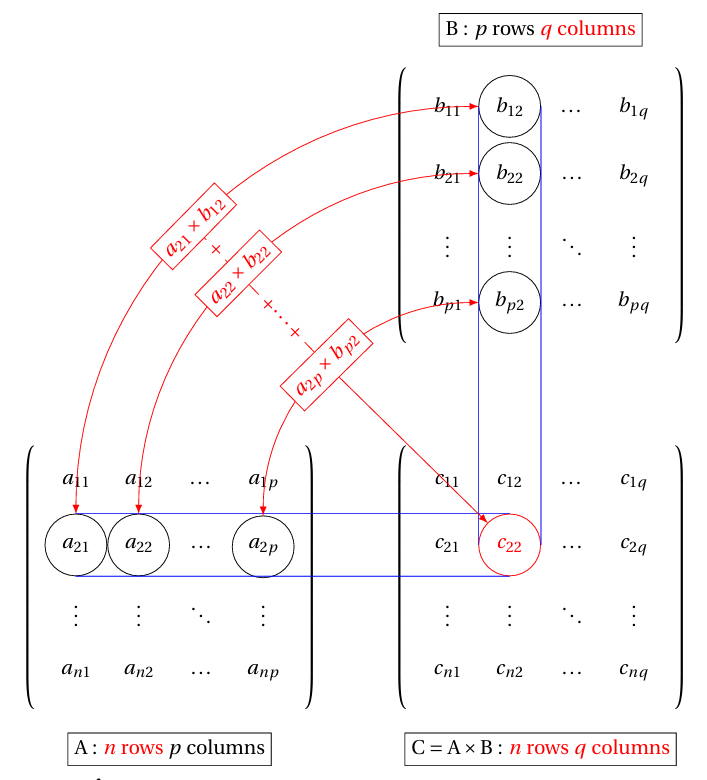
\includegraphics[width=6cm, height=6cm]{Slides/Figure/matricemultiplication.png}
\end{figure}
\end{frame}
\begin{frame}
    \frametitle{Ví dụ}
    Tính tích \[\begin{bmatrix}
    1&5\\ 3&2
\end{bmatrix}\begin{bmatrix}
    2&-1\\ 0&3
\end{bmatrix}\] theo hai cách: \eqref{eq4} và bằng góc nhìn của phép nhân vector.
\end{frame}
\begin{frame}
    \frametitle{Ví dụ- Giải}
    Cách 1: \[\begin{bmatrix}
    (1\cdot 2+5\cdot 0)&(1\cdot -1+5\cdot 3)\\
   ( 3\cdot 2+2\cdot 0)&(3\cdot -1+2\cdot 3)
\end{bmatrix}=\begin{bmatrix}
    2&14\\
    6&3
\end{bmatrix}.\]
\end{frame}
\begin{frame}
    \frametitle{Ví dụ-Giải}
    Cách 2: Theo góc nhìn của phép nhân vector, tích này tương đương với 
\[\begin{bmatrix}
    \begin{bmatrix}
        1&5\\3&2
    \end{bmatrix}\begin{bmatrix}
        2\\0
    \end{bmatrix} &\begin{bmatrix}
        1&5\\3&2
    \end{bmatrix}\begin{bmatrix}
        -1\\3
    \end{bmatrix}
\end{bmatrix}.\]
Dễ thấy, \begin{align*}
    &\begin{bmatrix}
        1&5\\3&2
    \end{bmatrix}\begin{bmatrix}
        2\\0
    \end{bmatrix}=2\begin{bmatrix}
        1\\3
    \end{bmatrix}+0\begin{bmatrix}
        5\\2
    \end{bmatrix}=\begin{bmatrix}
        2\\6
    \end{bmatrix},\\
    &\begin{bmatrix}
        1&5\\3&2
    \end{bmatrix}\begin{bmatrix}
        -1\\3
    \end{bmatrix}=-1\begin{bmatrix}
        1\\3
    \end{bmatrix}+3\begin{bmatrix}
        5\\2
    \end{bmatrix}=\begin{bmatrix}
        14\\3
    \end{bmatrix}.
\end{align*}
\end{frame}
\begin{frame}
    \frametitle{Các phép toán trên ma trận}
    \textbf{Các quy tắc cho các phép toán trên ma trận.} Ta tổng kết lại các quy tắc chung nhất.
    \begin{enumerate}
    \item Quy luật giao hoán: \(\mathbf{A}+\mathbf{B}=\mathbf{B}+\mathbf{A}\).
    \item Quy luật phân phối: \(\alpha(\mathbf{A}+\mathbf{B})=\alpha\mathbf{A}+\alpha\mathbf{B}\).
    \item Quy luật liên kết: \(\mathbf{A}+(\mathbf{B}+\mathbf{C})=(\mathbf{A}+\mathbf{B})+\mathbf{C}\).
    \item Quy luật liên kết: \((\mathbf{AB})\mathbf{C}=\mathbf{A}(\mathbf{BC})\).
    \item Quy luật phân phối (trái): \(\mathbf{A}(\mathbf{B}+\mathbf{C})=\mathbf{AB}+\mathbf{AC}\).
    \item Quy luật phân phối (phải): \((\mathbf{A}+\mathbf{B})\mathbf{C}=\mathbf{AC}+\mathbf{BC}\).
    \item Quy luật giao hoán: \(\mathbf{AB} \neq \mathbf{BA}\).
\end{enumerate}
Chú ý quy luật cuối cùng, tích ma trận không mang tính giao hoán.
\end{frame}
\subsection{Phép biến đổi tuyến tính}
\begin{frame}
    \frametitle{Hệ phương trình tuyến tính}
    Một hệ hai phương trình tuyến tính ở dạng tổng quát:
\begin{align*}
a_{11}x_{1} + a_{12}x_{2} &= b_{1}, \\
a_{21}x_{1} + a_{22}x_{2} &= b_{2}.
\end{align*}
Tương đương với,
\[\begin{bmatrix}
    a_{11}\\a_{21}
\end{bmatrix}x_{1}+\begin{bmatrix}
    a_{12}\\a_{22}
\end{bmatrix}x_{2}=\begin{bmatrix}
    b_{1}\\b_{2}
\end{bmatrix};\]
\[\begin{bmatrix}
    a_{11}&a_{12}\\
    a_{21}&a_{22}
\end{bmatrix}\begin{bmatrix}
    x_{1}\\x_{2}
\end{bmatrix}=\begin{bmatrix}
    b_{1}\\b_{2}
\end{bmatrix}.\]
Hệ phương trình tuyến tính được gói gọn thành 
\[\mathbf{A}\mathbf{x}=\mathbf{b}.\]
\end{frame}
\begin{frame}
    \frametitle{Nghiệm của hệ phương trình tuyến tính}
    Nghiệm của hệ phương trình tuyến tính đó ở dạng tổng quát:
    \begin{align*}
x_{1} &= a_{11}^{-1}b_{1} + a_{12}^{-1}b_{2}, \\
x_{2} &= a_{21}^{-1}b_{1} + a_{22}^{-1}b_{2}.
\end{align*}
Viết lại trong ngôn ngữ của vector:
\[\begin{bmatrix}
    x_{1}\\x_{2}
\end{bmatrix}=\begin{bmatrix}
    a_{11}^{-1}&a_{12}^{-1}\\
    a_{21}^{-1}&a_{22}^{-1}
\end{bmatrix}\begin{bmatrix}
    b_{1}\\b_{2}
\end{bmatrix}.\]
\[\implies \mathbf{x}=\mathbf{A}^{-1}\mathbf{b}\]
\(\mathbf{A}^{-1}\) được gọi là ma trận nghịch đảo của \(\mathbf{A}\).
\end{frame}
\begin{frame}
    \frametitle{Phép biến đổi}
    \begin{center}
\begin{tabular}{|c|c|c|}
  \hline
   & Ma trận & Hàm số \\
  \hline
  Dạng chuẩn & \(\mathbf{A}\mathbf{x}=\mathbf{b}\) & \(f(x)=y\) \\
  \hline
   Nghịch đảo& \(\mathbf{x}=\mathbf{A}^{-1}\mathbf{b}\) & \(x=f^{-1}(y)\) \\
  \hline
\end{tabular}
\end{center}
\end{frame}
\begin{frame}
    \frametitle{Phép biến đổi}
    \begin{center}
\begin{tabular}{|c|c|c|}
  \hline
   & Ma trận & Hàm số \\
  \hline
  Dạng chuẩn & \(\mathbf{A}\mathbf{x}=\mathbf{b}\) & \(f(x)=y\) \\
  \hline
   Nghịch đảo& \(\mathbf{x}=\mathbf{A}^{-1}\mathbf{b}\) & \(x=f^{-1}(y)\) \\
  \hline
\end{tabular}
\end{center}
Hàm của vector? Phép biến đổi.
\[T: \mathbb{R}^n \rightarrow \mathbb{R}^m,\]
\[\mathbf{u}\rightarrow T(\mathbf{u})=\mathbf{v}.\]
\end{frame}
\begin{frame}
    \frametitle{Phép biến đổi}
    Vậy là, ta luôn có \[T(\mathbf{x})=\mathbf{A}\mathbf{x}?\]
\end{frame}
\begin{frame}
    \frametitle{Phép biến đổi}
    Câu trả lời là khôn, với một phép biến đổi phi tuyến, chẳng hạn:
    \[T\left(\begin{bmatrix}
    x_1\\x_2
\end{bmatrix}\right)=\begin{bmatrix}
    x_{1}^2 +x_{2}^2 \\x_{1}^2 -x_{2}^2
\end{bmatrix}.\]
\end{frame}
\begin{frame}
    \frametitle{Phép biến đổi tuyến tính}
    \begin{center}
\begin{tabular}{|c|c|c|}
  \hline
   & Ma trận & Hàm số \\
  \hline
  Dạng chuẩn & \(\mathbf{A}\mathbf{x}=\mathbf{b}\) & \(f(x)=y\) \\
  \hline
   Nghịch đảo& \(\mathbf{x}=\mathbf{A}^{-1}\mathbf{b}\) & \(x=f^{-1}(y)\) \\
  \hline
  Tính tuyến tính & \(\mathbf{A}(\mathbf{x}_1+\mathbf{x}_2)=\mathbf{A}\mathbf{x}_1 +\mathbf{A}\mathbf{x}_2\) &\(f(x_1 +x_2)=f(x_1)+f(x_2)\)\\
  Tính đồng nhất & \(\mathbf{A}(\alpha\mathbf{x})=\alpha\mathbf{A}\mathbf{x}\)&\(f(\alpha x)=\alpha f(x)\)\\
  \hline
\end{tabular}
\end{center}
\end{frame}
\begin{frame}
    \frametitle{Phép biến đổi tuyến tính}
    \begin{tcolorbox}[colback=blue!10, colframe=blue!50!black, title=Định nghĩa]
        Một biến đổi tuyến tính là biến đổi \(L: \mathbb{R}^n \rightarrow\mathbb{R}^m\) thoả mãn hai đặc tính:
    \[\text{tuyến tính:}\quad L(\mathbf{u}+\mathbf{v})=L(\mathbf{u})+L(\mathbf{v}),\]
    \[\text{tuyến tính:}\quad L(\alpha\mathbf{v})=\alpha L(\mathbf{v}).\]
    \end{tcolorbox}
    \begin{enumerate}
    \item \(L(\mathbf{0})=\mathbf{0}\).
    \item \(L(\alpha_{1}\mathbf{e}_1+\alpha_2 \mathbf{e}_2 +\cdots +\alpha_n \mathbf{e}_{n})=\alpha_1 L(\mathbf{e}_1)+\alpha_2 L(\mathbf{e}_2)+\cdots +\alpha_n L(\mathbf{e}_n)\).
\end{enumerate}
\end{frame}
\begin{frame}
    \frametitle{Ma trận chuẩn của phép biến đổi}
    \begin{equation}
        L(\mathbf{x})=\begin{bmatrix}
    \lvert & \lvert &\lvert &\lvert\\
    L(\mathbf{e}_1)&L(\mathbf{e}_2)&\cdots&L(\mathbf{e}_n)\\
     \lvert & \lvert &\lvert &\lvert
\end{bmatrix}\begin{bmatrix}
    \alpha_1 \\\alpha_2 \\\vdots\\ \alpha_n
\end{bmatrix}.
    \end{equation}
Rút gọn,
    \[L(\mathbf{x})=\mathbf{A}\mathbf{x},\]
    với \(\mathbf{A}\) được gọi là ma trận chuẩn của phép biến đổi.
\end{frame}
\begin{frame}
    \frametitle{Ví dụ}
    Tìm ma trận của phép biến đổi 
    \[L\left(\begin{bmatrix}
    x_1 \\x_2
\end{bmatrix}\right)=\begin{bmatrix}
    x_1 +2x_2 \\x_2
\end{bmatrix},\]
và tính toạ độ \(\mathbf{x}=(1,1)\) sau phép biến đổi.
\end{frame}
\begin{frame}
    \frametitle{Ví dụ}
    Áp dụng biến đổi này lên hai vector đơn vị \(\mathbf{e}_1 =(1,0)\) và \(\mathbf{e}_2 =(0,1)\):
\[\mathbf{e}_1 \rightarrow (1,0),\qquad \mathbf{e}_2 \rightarrow (2,1).\] Với vector \(\mathbf{x}=(1,1)\):
\[\mathbf{x}=\begin{bmatrix}
1\\1
\end{bmatrix}\rightarrow 1\begin{bmatrix}
1\\0
\end{bmatrix}+1\begin{bmatrix}
2\\1
\end{bmatrix}=\begin{bmatrix}
    1&2\\0&1
\end{bmatrix}\begin{bmatrix}
    1\\1
\end{bmatrix}=\begin{bmatrix}
    3\\1
\end{bmatrix}.\]
\end{frame}

\subsection{Minh hoạ cho phép biến đổi tuyến tính}
\begin{frame}
    \frametitle{Minh hoạ cho phép biến đổi tuyến tính}
    
    \begin{figure}[H]
        \centering
        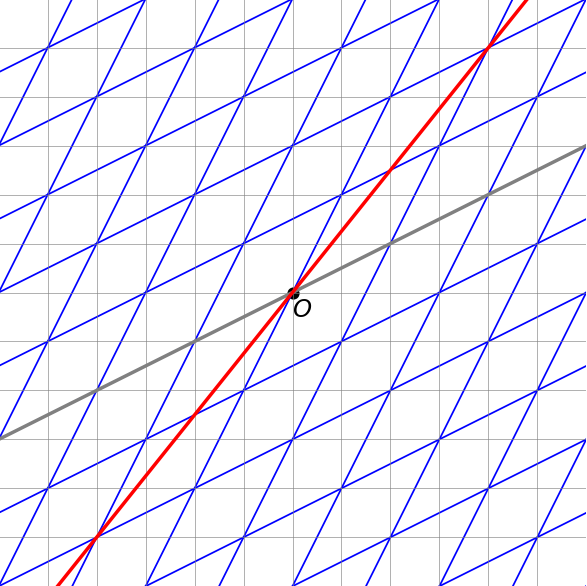
\includegraphics[width=7cm, height=5cm]{Slides/Figure/LT1.png}
    \end{figure}
 \[\mathbf{A}=\begin{bmatrix}
        1&2\\2&1
    \end{bmatrix}\]
\end{frame}
\begin{frame}
    \frametitle{Tiêu chí cho hình ảnh của lưới cho một phép biến đổi tuyến tính}
    \begin{itemize}
    \item Điểm O giữa nguyên vị trí.
    \item Các đường kẻ của lưới song song và cách đều nhau.
    \item Một đường thẳng vẫn là một đường thẳng.
\end{itemize}
\begin{figure}[H]
        \centering
        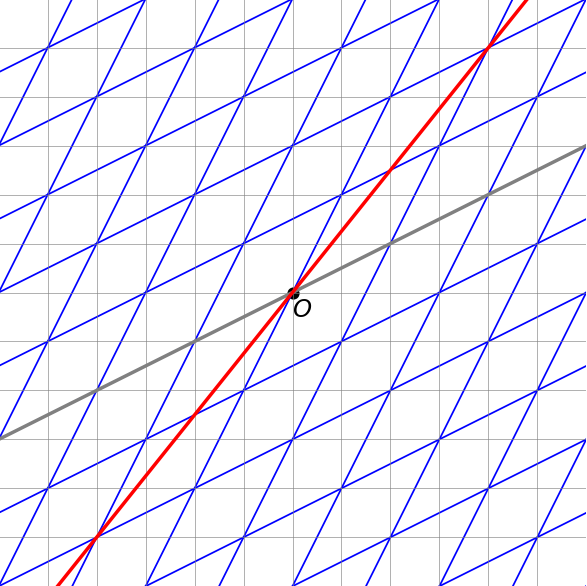
\includegraphics[width=6cm, height=4cm]{Slides/Figure/LT1.png}
    \end{figure}
\end{frame}
\begin{frame}
    \frametitle{Minh hoạ cho một phép biến đổi tuyến tính}
    \[\mathbf{v}=\begin{bmatrix}
    1\\0.5
\end{bmatrix}\rightarrow L\rightarrow L(\mathbf{v})=\begin{bmatrix}
    2\\2.5
\end{bmatrix}.\]
    \begin{figure}[H]
        \centering
        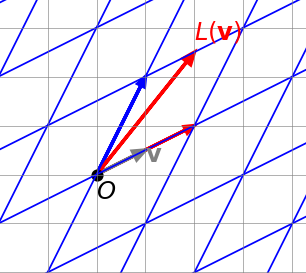
\includegraphics[width=6cm, height=4cm]{Slides/Figure/LT2.png}
    \end{figure}
\end{frame}
\begin{frame}
    \frametitle{Phép biến đổi cắt}
    \[\mathbf{A}=\begin{bmatrix}
        1&2\\0&1
    \end{bmatrix}\]
    \begin{figure}
        \centering
        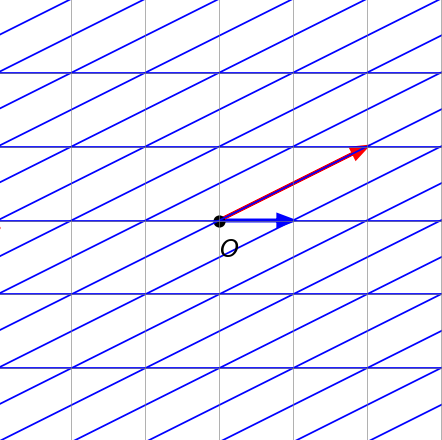
\includegraphics[width=5cm, height=4cm]{Slides/Figure/LT3.png}
    \end{figure}
\end{frame}
\begin{frame}
    \frametitle{Phép biến đổi cắt}
    Phương trình cho một biến đổi cắt 2D :
\[
L\left(\begin{bmatrix}
    x_1 \\x_2
 \end{bmatrix}\right)=\begin{bmatrix}
    x_1 +\lambda x_2 \\x_2
 \end{bmatrix}, \text{ hoặc}\quad 
 \begin{bmatrix}
    x_1 \\\lambda x_1 +x_2
 \end{bmatrix}.\]
Ma trận biến đổi đặc trưng
\[\begin{bmatrix}
    1&\lambda\\0&1
\end{bmatrix},\] hoặc 
\[\begin{bmatrix}
    1&0\\\lambda&1
\end{bmatrix}.\]
\end{frame}
\begin{frame}
    \frametitle{Phép giãn nở}
    \[\mathbf{D}=
    \begin{bmatrix}
        3&0\\0&5
    \end{bmatrix}\]
    \begin{figure}
        \centering
        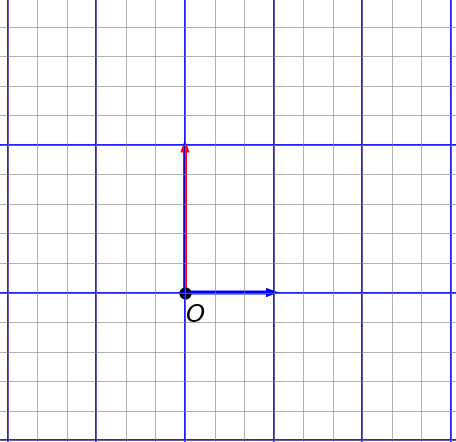
\includegraphics[width=5cm, height=4cm]{Slides/Figure/LT6.png}
    \end{figure}
\end{frame}
\begin{frame}
\frametitle{Phép giãn nở}
    Biến đổi cho một giãn nở 2D là 
\[L\left(\begin{bmatrix}
    x_1 \\x_2
\end{bmatrix}\right)=\begin{bmatrix}
    \lambda_1 x_1 \\\lambda_2 x_2
\end{bmatrix}.\]
Ma trận biến đổi là một ma trận đường chéo:
\[\mathbf{D}=\begin{bmatrix}
    \lambda_1 &0\\0&\lambda_2
\end{bmatrix}.\]
Chú ý, \[\mathbf{D}^{-1}=\begin{bmatrix}
    \lambda_{1}^{-1} &0\\0&\lambda_{2}^{-1}
\end{bmatrix}.\]
\end{frame}
\begin{frame}
    \frametitle{Phép quay}
    \begin{figure}[H]
        \centering
        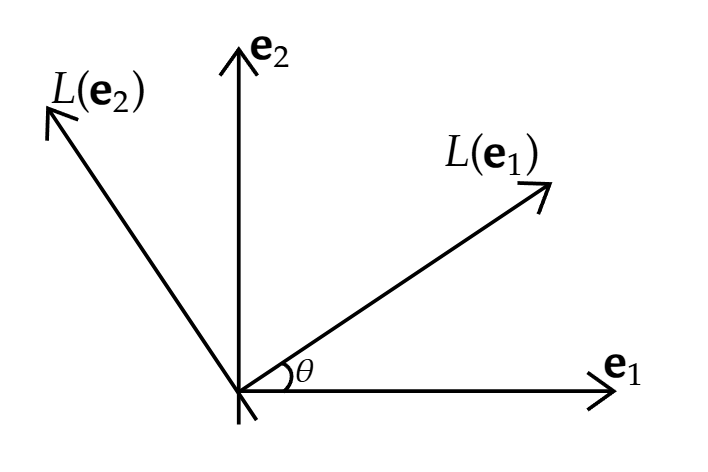
\includegraphics[width=6cm, height=4cm]{Slides/Figure/rotation.png}
    \end{figure}
    \[\mathbf{R}=\begin{bmatrix}
    \cos\theta &-\sin\theta\\
    \sin\theta &\cos\theta
\end{bmatrix};\qquad \mathbf{R}^{-1}=\mathbf{R}^T .\]
\end{frame}
\begin{frame}
    \frametitle{Phép quay}
    \begin{columns}
        \begin{column}{0.5\textwidth}
            \begin{figure}[H]
                \centering
                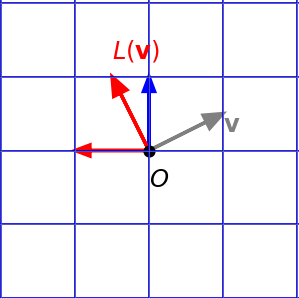
\includegraphics[width=3cm, height=3cm]{Slides/Figure/LT7.png}
            \end{figure}
            Phép quay 90 độ theo chiều dương
            \[\mathbf{R}=\begin{bmatrix}
                0&-1\\1&0
            \end{bmatrix}.\]
        \end{column}
        \begin{column}{0.5\textwidth}
            \begin{figure}[H]
                \centering
                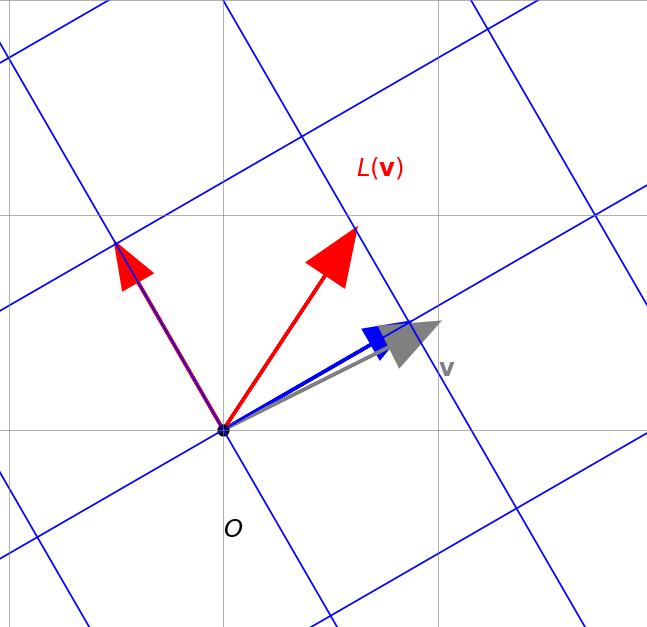
\includegraphics[width=3cm, height=3cm]{Slides/Figure/LT8.png}
            \end{figure}
            Phép quay 30 độ theo chiều dương
        \end{column}
    \end{columns}
\end{frame}
\begin{frame}
    \frametitle{Phép quay}
    \begin{figure}[H]
        \centering
        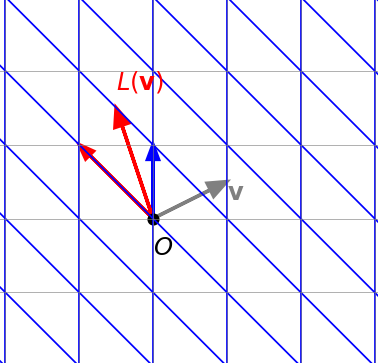
\includegraphics[width=5cm, height=4cm]{Slides/Figure/LT9.png}
    \end{figure}
    Kéo rồi quay 90 độ:
    \[\begin{bmatrix}
        0&-1\\1&0
    \end{bmatrix}\begin{bmatrix}
        1&1\\0&1
    \end{bmatrix}.\]
\end{frame}
\subsection{Chuyển cơ sở}
\begin{frame}
    \frametitle{Chuyển cơ sở}
    \begin{columns}
        \begin{column}{0.5\textwidth}
            Hai hệ cơ sở:
               \begin{itemize}
                  \item Hệ \(\mathcal{A}:\{\mathbf{e}_1 ,\mathbf{e}_2\}\) 
                \item Hệ \(\mathcal{B}:\{\mathbf{e}_3 ,\mathbf{e}_4\}\) 
                \end{itemize}
    Trong hệ \(\mathcal{A}\), \[\mathbf{v}_{\mathcal{A}}=\begin{bmatrix}
    5\\3
\end{bmatrix}.\] Trong hệ \(\mathcal{B}\), \[\mathbf{v}_{\mathcal{B}}=\begin{bmatrix}
    1\\3
\end{bmatrix}.\]
        \end{column}
        \begin{column}{0.5\textwidth}
            \begin{figure}
                \centering
                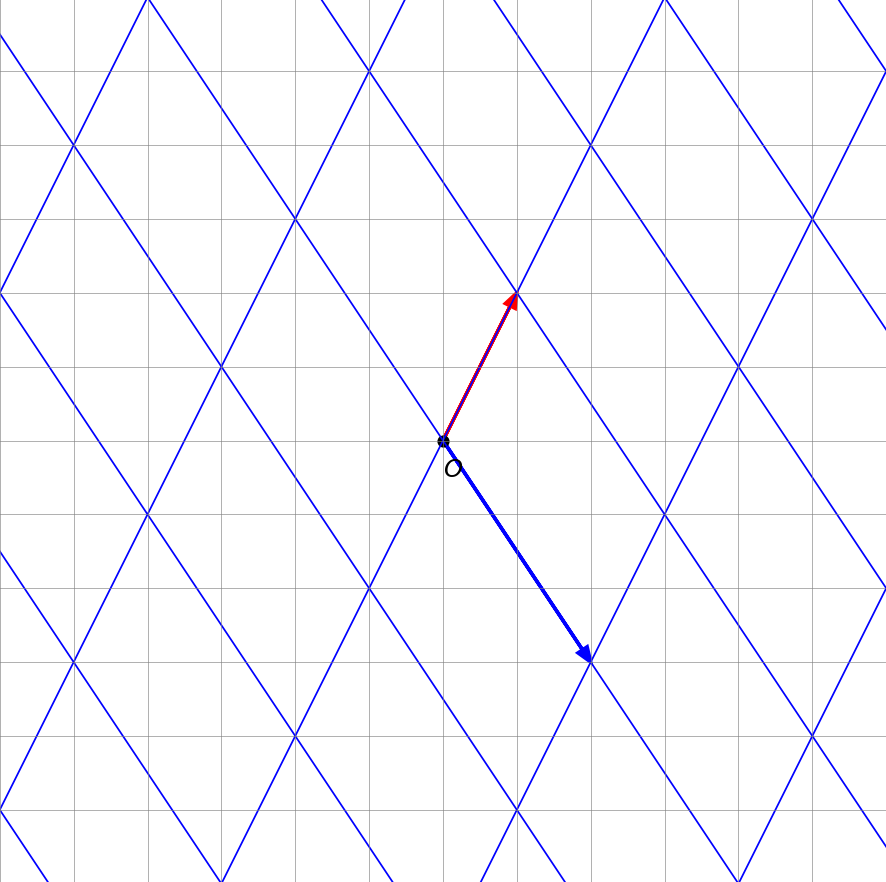
\includegraphics[width=7cm, height=5cm]{Slides/Figure/LT10.png}
            \end{figure}
        \end{column}
    \end{columns}
\end{frame}
\begin{frame}
    \frametitle{Chuyển cơ sở}
    \begin{columns}
        \begin{column}{0.5\textwidth}
            Biết rằng
           \[\mathbf{e}_3 =2\mathbf{e}_1 +(-3)\mathbf{e}_4 ,\quad \mathbf{e}_4 =1\mathbf{e}_1 +2\mathbf{e}_2 .\]
           Ta thu được gì?
          \[\begin{bmatrix}
    2&1\\-3&2
\end{bmatrix}\begin{bmatrix}
    1\\3
\end{bmatrix}=\begin{bmatrix}
    5\\3
\end{bmatrix},\] tức là
\[\mathbf{P}\mathbf{v}_{\mathcal{B}}=\mathbf{v}_{\mathcal{A}}.\]
        \end{column}
        \begin{column}{0.5\textwidth}
            \begin{figure}
                \centering
                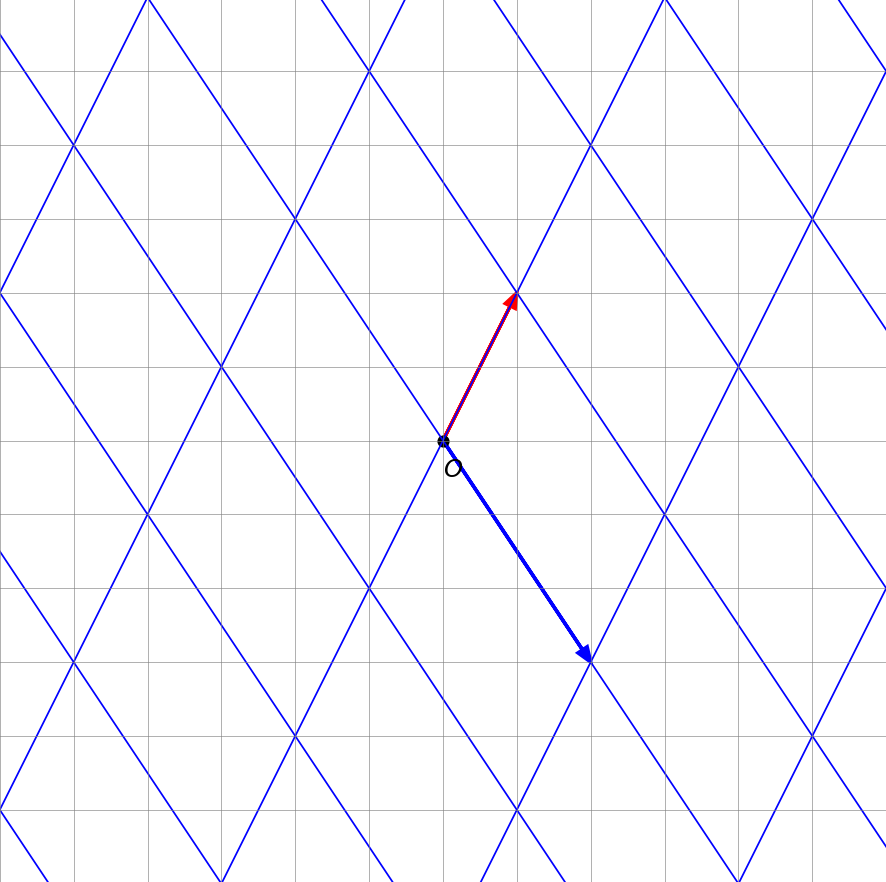
\includegraphics[width=7cm, height=5cm]{Slides/Figure/LT10.png}
            \end{figure}
        \end{column}
    \end{columns}
\end{frame}
\begin{frame}
    \frametitle{Chuyển cơ sở}
    \begin{columns}
        \begin{column}{0.5\textwidth}
        

          \[\mathbf{P}(\mathbf{e}_1)_{\mathcal{A}}=\mathbf{P}(\mathbf{e}_3)_{\mathcal{B}}=(\mathbf{e}_3)_{\mathcal{A}},\]
\[\mathbf{P}(\mathbf{e}_2)_{\mathcal{A}}=\mathbf{P}(\mathbf{e}_4)_{\mathcal{B}}=(\mathbf{e}_4)_{\mathcal{A}}.\] 
        \end{column}
        \begin{column}{0.5\textwidth}
            \begin{figure}
                \centering
                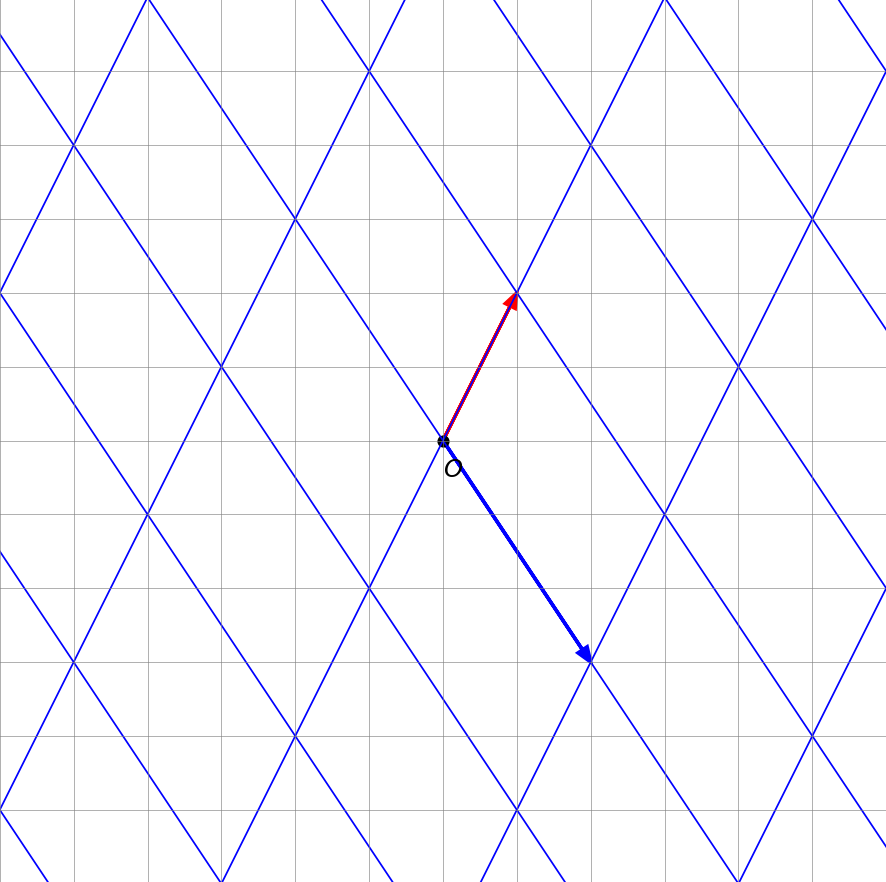
\includegraphics[width=7cm, height=5cm]{Slides/Figure/LT10.png}
            \end{figure}
        \end{column}
    \end{columns}
\end{frame}
\begin{frame}
    \frametitle{Chuyển cơ sở}
            \begin{equation*}
                \mathbf{P}\mathbf{v}_{\mathcal{B}}=\mathbf{v}_{\mathcal{A}}.
            \end{equation*}
        \begin{equation*}
            \mathbf{P}^{-1}\mathbf{v}_{\mathcal{A}}=\mathbf{v}_{\mathcal{B}}.
        \end{equation*}
                \begin{figure}[H]
        \centering
        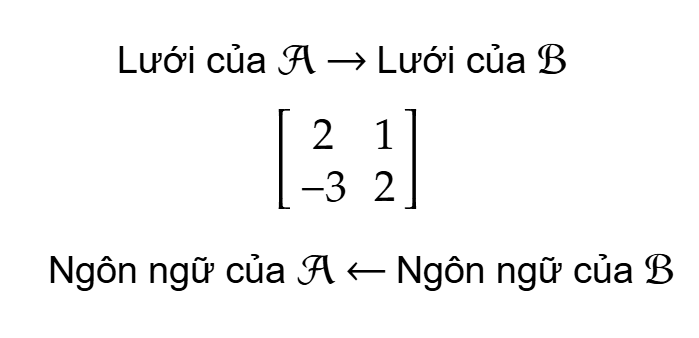
\includegraphics[width=7cm, height=4cm]{Slides/Figure/final.png}
    \end{figure}

\end{frame}
\begin{frame}
    \frametitle{Ví dụ}
    Một đường tròn bán kính \(R\) lăn không trượt với tốc độ không đổi, nghĩa là toạ độ của tâm đường tròn được cho bởi \((R\theta,R)\). Hãy xác định toạ độ của điểm M trong hệ toạ độ \(Oxy\), biểu diễn kết quả theo tham số \(\theta\).
\begin{figure}[H]
    \centering
    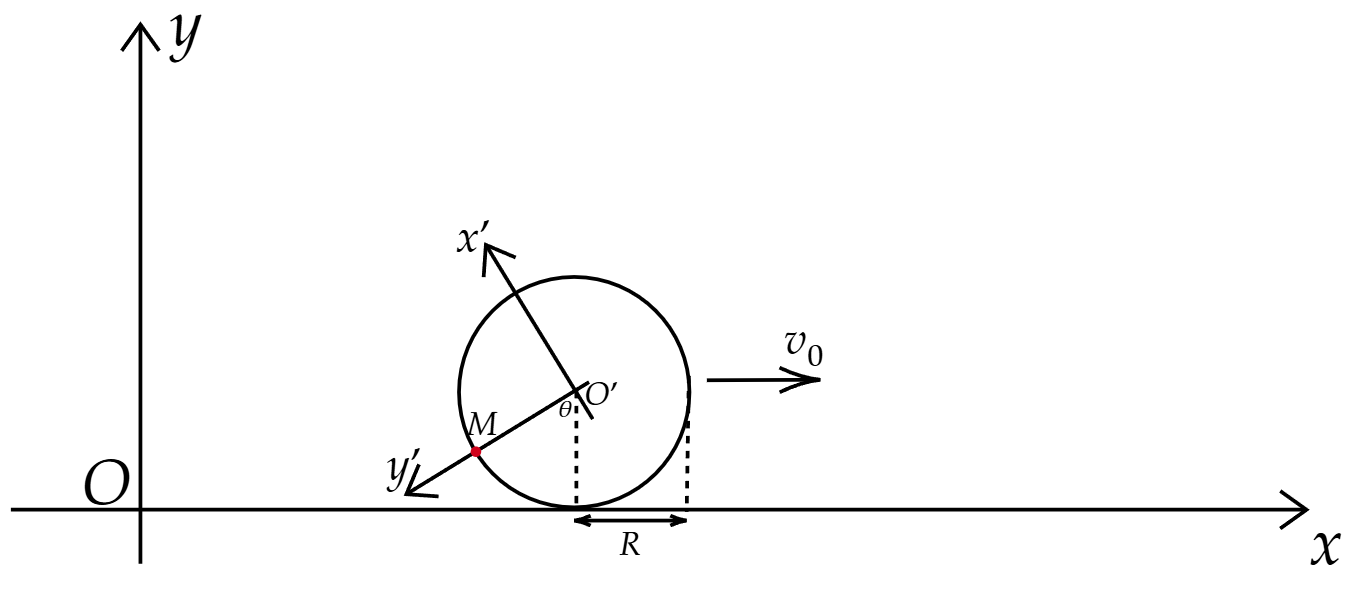
\includegraphics[width=9cm, height=4cm]{Slides/Figure/cycloidexample.png}
\end{figure}
\end{frame}
\begin{frame}
    \frametitle{Giải}
\[\begin{bmatrix}
    x\\y
\end{bmatrix}=\begin{bmatrix}
    \cos\phi&-\sin\phi \\\sin\phi&\cos\phi
\end{bmatrix}\begin{bmatrix}
    x'\\y'
\end{bmatrix}+\begin{bmatrix}
    R\theta\\R
\end{bmatrix},\] với \(\phi=\pi-\theta.\) Như vậy, 
\[\begin{bmatrix}
    x\\y
\end{bmatrix}=R\begin{bmatrix}
    \theta-\sin\theta\\1-\cos\theta
\end{bmatrix}.\] Quỹ đạo của điểm M chính là đường Cycloid.
\end{frame}

\subsection{Một số ví dụ khác về không gian vector}
\end{document}